\documentclass[conference]{IEEEtran}
	\pdfpagewidth=8.5truein
	\pdfpageheight=11truein

\usepackage{graphicx}
\usepackage{subfig}
\usepackage[bookmarks=false]{hyperref}
\usepackage{xspace}
\usepackage{listings}
\usepackage[usenames, dvipsnames]{color}
\usepackage{amssymb}


\usepackage{booktabs}         

\graphicspath{{./img/}}

%\hyphenation{op-tical net-works semi-conduc-tor}

%
\def\sharedaffiliation{%
\end{tabular}
\begin{tabular}{c}}
%

\lstset{language=Python}

\definecolor{LightGray}{RGB}{250,250,250}

\lstdefinestyle{custompython}{
	captionpos=b,                    % sets the caption-position to bottom
	% frame=tb,
	xleftmargin=\parindent,
	language=Python,
	basicstyle=\footnotesize\ttfamily,
	keywordstyle=\bfseries\color{MidnightBlue},
	morekeywords={*,python,times,test_folder,url},
	stringstyle=\color{PineGreen},
  	commentstyle=\color{Magenta},
  	backgroundcolor=\color{LightGray}
}


\newcommand{\tool}{Flask Dashboard\xspace}
\newcommand{\zee}{Zeeguu\xspace}
\newcommand{\git}{\texttt{git}\xspace}
\newcommand{\install}{{\small \texttt{pip install flask\_monitoring\_dashboard}}\xspace}
\newcommand{\activeUserCount}{two hundred\xspace}
\newcommand{\code}[1]{\texttt{#1}\xspace}
\newcommand{\perspective}[1]{{\bf {\small {\texttt{#1}}\xspace}}}

\newcommand{\lesson}[1]{{\bf {\small {\texttt{Lesson: }}\xspace}}: #1}

\usepackage{fourier-orns}

\definecolor{myred}{RGB}{230, 20, 70}
\definecolor{mygreen}{RGB}{60, 180, 75}
\definecolor{uploadUserData}{RGB}{135, 143, 197}
\definecolor{feedItems}{RGB}{245, 130, 48}


\newcommand{\niceseparator}
	{
		\begin{center}
  		% $\ast$~$\ast$~$\ast$
  		% $\clubsuit$~$\clubsuit$~$\clubsuit$
  		\leafleft
		\end{center}
	}

% Endpoint Names 
%\newcommand{\epDecoration}[1]{{\small {\bf #1}}\xspace}
\newcommand{\epDecoration}[1]{\code{#1}}

\newcommand{\epColorDecoration}[2]{\color{#1}$\blacksquare$\color{black}\code{#2}}

\newcommand{\epTranslations}{{\epColorDecoration{myred}{api.get\_possible\_translations}}\xspace}
\newcommand{\epOutcome}{\epColorDecoration{mygreen}{api.report\_exercise\_outcome}}
\newcommand{\epFeedItems}{\epColorDecoration{feedItems}{api.get\_feed\_items\_with\_metrics}}
\newcommand{\epUserActivity}{\epColorDecoration{uploadUserData}{api.upload\_user\_activity\_data}}


% Author Comments / Discussion

\definecolor{mlcolor}{RGB}{140, 140, 205}
\definecolor{vacolor}{RGB}{255, 0, 255}

\newcommand{\ml}[1]{ 
	{\footnotesize \color{mlcolor}ML: #1}
	}

\newcommand{\ins}[1]{ 
	{\color{blue}#1}
	}


\newcommand{\va}[1]{ 
	{\footnotesize \color{vacolor}VA: #1}
}


\newcommand{\mltp}[1]{\ml{Thijs, Patrick: #1}}
\newcommand{\mlv}[1]{\ml{Vasilios: #1}}

\definecolor{todocolor}{RGB}{200, 140, 200}

\newcommand{\todo}[1]{ 
	{\bfseries \color{todocolor}Todo: #1}
	}

\newcommand{\Fref}[1]{Fig.~\ref{#1}}
\newcommand{\Sref}[1]{Sec.~\ref{#1}}




\begin{document}
	

%
\title{Agile Monitoring of Evolving Web Services: For the Little Man}

\author{
\IEEEauthorblockN{Author One, Author Two, Author Three}\\
Famous Institute for Software Engineering and Computer Science\\
University of Great City, Some Country\\
Email: \{first.last\}@university.to 
}


% make the title area
\maketitle

%!TEX root=paper.tex

\begin{abstract}
  Python is one of the fastest growing programming languages of the moment. Flask, a Python-based web framework is the technology chosen by tens of thousands of web applications. Many of these Flask-based projects are small websites which can not afford to deploy an advanced service monitoring solution because they are too complicated to install. Many of these projects might offer a service API. Given the complexity of professional monitoring tools it is very likely that 

  In this paper, we set out to show how to design a dashboard for a Flask API which is useful in understanding and guiding service evolution while at the same time, requiring minimal configuration and installation. We present \tool, a tool that provide insight into the utilization and performance of evolving services. We present the ease with which the library can be integrated in an already existing web application, discuss some of the visualization perspectives that the library provides and point to some future challenges for similar libraries.

\end{abstract}




\section{Introduction}

\todo{Intro to be rewritten; refer to VISSOFT paper as previous work, explain focus is on integration with version control/CI for evolution support, and use of unit tests as early performance indicator}

\todo{motivate with: monitoring in a world which is becoming more and more service-oriented is essential because it allows to perform three main types of actions: system adaptations to provide the request service at the desired level of quality, enabling flexibility in dealing with changing requirements and modes of operation, and enabling operational awareness through dashboards organizing the collected data~\cite{pernici2016monitoring}. In this work we focus on the last part and we discuss how a minimal effort probe-based solution for a particular type of web services can be used to facilitate the other two types of actions by involving the developer.}

\todo{explain: in~\cite{vogel2017low} we introduced the \tool an a high level with a focus on presenting its performance visualization aspects; in this work we only summarize these features by means of introducing some of the provided functionalities of the \tool. We focus on discussing how the tool is implemented and operating, provide a deeper look at its capabilities for integration with version control and continuous integration environments, introduce a mechanism for performance prediction, and provide an evaluation of the proposed approach based on a case study. }

%Every system is a distributed system nowadays \cite{cavage2013there}. Indeed a very large number of applications and web applications are nowadays implemented as two-tier architectures with a front-end implemented with web technologies and a service back-end.
%\ml{I'm not completely happy with this paragraph}
{\em There is no getting around it: you are building a distributed system} argues a recent article \cite{cavage2013there}. Indeed, even the simplest second-year student project is a web application implemented as two-tier architecture with a Javascript/HTML5 front-end a service backend, usually a REST API.

% \hfill mds
% Many contemporary programming languages are offering libraries, modules, or frameworks that facilitate the development of such architectures. 
Python is one of the most popular programming language choices for implementing the back-end of web applications. GitHub contains more than 500K open source Python projects and the Tiobe Index\footnote{TIOBE programming community index is a measure of popularity of programming languages, created and maintained by the TIOBE Company based in Eindhoven, the Netherlands} ranks Python as the 4th most popular programming language as of June 2016. An analysis of  StackOverflow from September 2017 argues that {\em ``Python has a solid claim to being the fastest-growing major programming language''}\footnote{https://stackoverflow.blog/2017/09/06/incredible-growth-python/}.
 
% possible flask summary
Within the Python community, Flask\footnote{\url{http://flask.pocoo.org/}} is a very popular web framework\footnote{More than 25K projects on GitHub (5\% of all Python projects) are implemented with Flask (cf. a GitHub search for ``language:Python Flask'')}. It provides simplicity and flexibility by implementing a bare-minimum web server, and thus advertises as a micro-framework. The Flask tutorial shows how setting up a simple Flask {\em ``Hello World''} web-service requires no more than 5 lines of Python code \cite{ flask:tutorial}.
% end of summary
 
Despite their popularity, to the best of our knowledge, there is no simple solution for monitoring the evolving performance of Flask web applications. Thus, every one of the developers of these projects faces one of the following options when confronted with the need of gathering insight into the runtime behavior of their implemented services: 

  \begin{enumerate}

    \item Use a commercial monitoring tool which treats the subject API as a black-box (e.g. Pingdom, Runscope). 
    % , Graphite+Graphana+statd etc.

    \item Implement their own ad-hoc analytics solution, having to reinvent basic visualization and interaction strategies. 

    \item Live without analytics insight into their services.

  \end{enumerate}

%\todo{For the first point in the list, we can also argue that analytics solutions like Google Analytics can be used, but they have no notion of versioning/integration with the development life cycle. Feel free to cite \cite{papazoglou2011managing} for service evolution purposes}

For projects on a budget (e.g. research, startups) the first and the second options are often not available due to time and financial constraints. Even when using 3rd-party analytics solutions, a critical insight into the evolution of the exposed services of the web application, is missing because such solutions have no notion of versioning and no integration with the development life cycle.~\cite{papazoglou2011managing}

To avoid projects ending up in the third situation, that of living without analytics, in this paper we present \tool~ --- a low-effort service monitoring library for Flask-based Python web services that is easy to integrate and enables the {\em agile assessment} of service evolution. \cite{Nier12b}

As a case study, on which we will illustrate our solution, we are going to use an open source API which, for several years, was in the third of the above-presented situations.

% In the next section, we will present a case study of an open source research API which was for a long time in the third situation presented above -- deployed without analytics insight.

\todo{Add signposting paragraph}



\section{Case Study: The API (Zeeguu)}
\label{sec:case}

%\todo{Either leave as is or add more info on usage by college if possible}

  \zee\footnote{\url{https://github.com/zeeguu-ecosystem/}} is a platform and an ecosystem of applications for accelerating vocabulary acquisition in a foreign language \cite{Lungu16}. 
%
  The architecture of the ecosystem has at its core an API and a series of satellite applications that together offer to a learner three main inter-dependent features:

  \begin{enumerate}

    \item Reader applications that provide effortless translations for those texts which are too difficult for the readers.

    \item Interactive exercises personally generated based on the preferences and past likes of the learner.

    \item Article recommendations which are personalized for the interests of the learner and come with difficulty estimation that helps the learner find articles with the appropriate difficulty.

  \end{enumerate}

  The core API implemented with Flask and Python provides correspondingly three types of functionality: contextual translations, article recommendations, and personalized exercise suggestions. In total the API provides a bit less than 50 endpoints, out of which probably a dozen are very frequently used. 
  % The development of the core API itself is a research project. 

  At the time of writing this article, the ecosystem consists of a reader web application, a web based exercises platform, and a smartwatch application, which are used at the moment of writing this article by more than \activeUserCount active users. The users come from a highschool, a language school, and some users are using it on their own, without any educational context. The highest load we observed until now on the API consisted of 12K requests in one day.

  \ml{add more numbers that show how impressive is our API}

  
  We will use this \zee API as a case study for this paper. 
  All the figures in this paper are captured from the actual deployment of \tool in the context of the \zee API. The figures are interactive offering basic data exploration capabilities: filter, zoom, and details on demand\cite{Shne99a}. The \tool deployment for the case study can be accessed publicly\footnote{\url{https://zeeguu.unibe.ch/api/dashboard}; username: {\em guest}, password: {\em soap-sac}}. 

 % \todo{create new account, update URL if necessary, update activeUserCount, add a couple of sentences of the current state of the case study with the college/language center}
% \ml{we should consider adding also one section in which the architecture/implementation and main features of the dashboard are presented before going on with discussing them in more depth in the following sections --- this should include a rundown on which views are provided from where (overview or per endpoint)}

\newpage



\section{Case Study: The Technology (Flask)}
\label{sec:tool}

 Flask is a microframework for Python. It IS USED BY THOUSANDS OF PROJECTS. ELABORATE MORE ON THIS... 
 \vspace{2cm}

 Flask depends on two external libraries: the Jinja2 template engine and the Werkzeug WSGI toolkit. 

 “Micro” does not mean that your whole web application has to fit into a single Python file (although it certainly can), nor does it mean that Flask is lacking in functionality. The “micro” in microframework means Flask aims to keep the core simple but extensible. Flask won’t make many decisions for you, such as what database to use. Those decisions that it does make, such as what templating engine to use, are easy to change. Everything else is up to you, so that Flask can be everything you need and nothing you don’t.

 Flask has many configuration values, with sensible defaults, and a few conventions when getting started. By convention, templates and static files are stored in subdirectories within the application’s Python source tree, with the names templates and static respectively. While this can be changed, you usually don’t have to, especially when getting started.

 A Python web application based on WSGI has to have one central callable object that implements the actual application. In Flask this is an instance of the Flask class. Each Flask application has to create an instance of this class itself and pass it the name of the module, but why can’t Flask do that itself?

\begin{lstlisting}[style=custompython]

from flask import Flask
app = Flask(__name__)

@app.route('/')
def index():
    return 'Hello World!'

\end{lstlisting}


\subsection*{ENSURE CLARITY: NOTHING PREVENTS GENERALIZATION}
In this article we take as an example the Flask case study
and of the \tool as a dashboard. 
But there is nothing that prevents the generalization of 
our approach to other languages and technologies. 




%!TEX root=paper.tex


  \newpage
  \section{Service Utilization and Performance}

  % Since it is tailored for Flask applications, the deployment of \tool is trivial. 

  The tool is designed to take advantage of the fact that it runs in the same web application context and that the monitored API already has a web presence. It thus simply makes available one extra endpoint (i.e. \code{/dashboard}) at the same address as the API, endpoint which serves the interactive application presented in the remainder of this paper. 

  A dashboard can be attached to an already existing Flask application with a single line of code as the code in the following snippet shows
  \footnote{We do not count the import statement that enables that line}:

  % which binds the dashboard to a Flask application\footnote{\ins{ In this paper we present the integration with APIs written in Python and Flask hoping that this will not prevent the reader from seeing the more general idea; all the tools we show here for Flask can be applied to other API technologies (e.g. Django) by simply providing a few back-end adapters in the right places. }}:

  % caption=Configuring the \tool is straightforward,
  \begin{lstlisting}[style=custompython]
  import flask_monitoringdashboard as dashboard

  # LOC #1: associate the main Flask application 
  # object with the dashboard
  dashboard.bind(app) 

  \end{lstlisting}

  During binding, the \tool will search for all endpoints defined in the target application and make them available in the dashboard in an interactive configuration panel (\Fref{fig:sep}). The panel presents all the automatically discovered endpoints and lets the user select the ones that should be monitored (the checkboxes in the last column). When the user enables the monitoring of an endpoint a function wrapper is added to the implementation of that endpoint (which is a function in Flask). The information is also saved in a database such that it is persistent across application restarts. 

  

  % In order to monitor an endpoint, the \tool creates a function wrapper for the API function that corresponds to the endpoint. This way, the wrapper will be executed whenever that API call is made before the actual function is called. The wrapper contains the code that takes care of monitoring an endpoint. 

    \begin{figure}[h!]
      \centering
      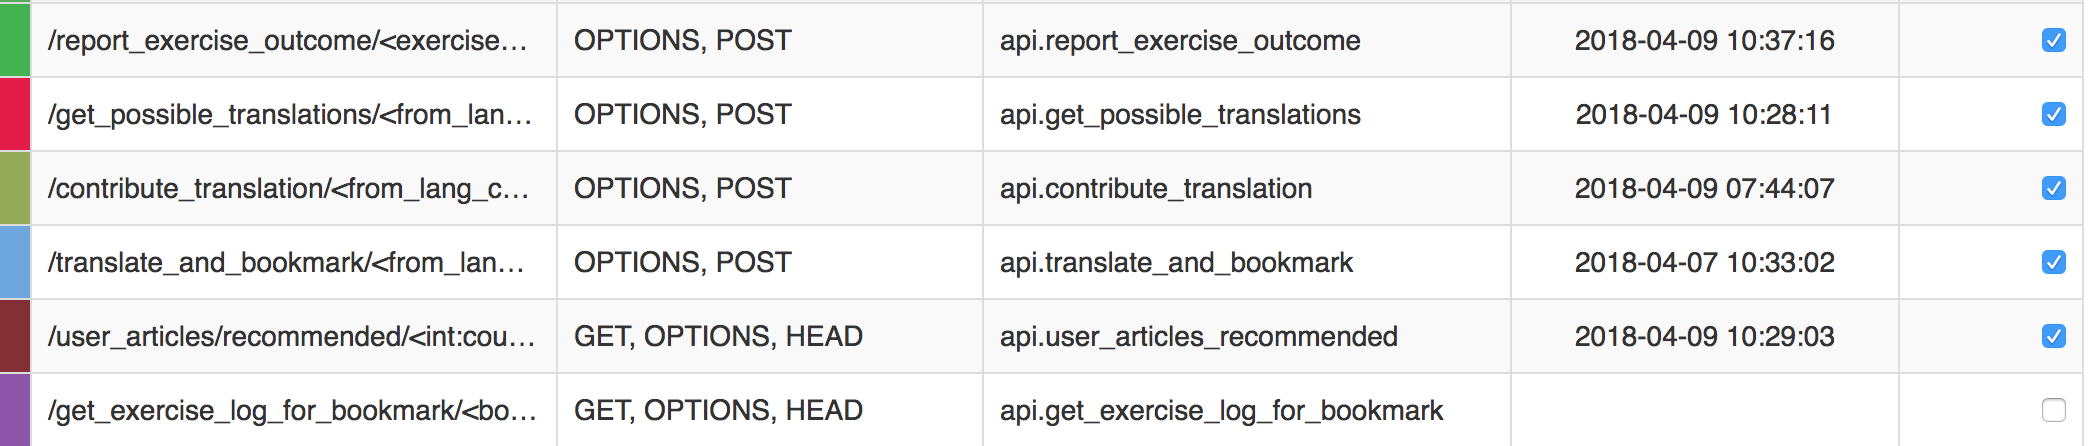
\includegraphics[width=\linewidth]{selecting_endpoints.png}
      \caption{Once connected to an API the Dashboard presents the endpoints that are available for monitoring}
      \label{fig:sep}
    \end{figure}

  By default the dashboard takes an {\em opt-in} approach to monitoring: to prevent the performance penalties incurred by the dashboard\footnote{We discuss performance issues later} to affect performance sensitive endpoints, the service developer is asked to manually add the endpoints they want to monitor. 
   

  One alternative to configuring the monitored endpoints from the user interface is to allow the service developer to annotate the code. This would however pollute the code, and prevent deploying two versions which would monitor different endpoints. Also, would pose problems with endpoint evolution in the future.

  
\niceseparator

  The remainder of this section presents several interactive
  visualizations that are available in the dashboared without any further configuration\footnote{We recommend obtaining a color version of this paper for better readability}. They are focused on two types of information that is important to the API maintainer: 

  \begin{itemize}

    \item {\bf Utilization} -- refers to how the third parties use the API, which parts are most used, which are little used, etc. This is known to be critical information for upstream developer in general\cite{Haen14a}. In the case of source code dependencies one can detect such information by analyzing software repositories. However, in the case of services, there is no other way but monitoring service utilization. 

    \item {\bf Performance} as measured in response times. This is important, especially for APIs that are supposed to be integrated in live systems. 

  \end{itemize}


%!TEX root=paper.tex


\newpage
\subsection{Utilization}
\label{sec:util}

\ins{Knowing how third parties use one's API is difficult even in the case of static dependencies. In the case of services, there is no other way but monitoring service utilization. \tool introduces a series of perspectives on utilization. }

\ins{
  
  The most basic possible view shows the cummulative information about all the endpoints and the number of calls to that endpoint over the lifetime of its tracking as well as in the current day and the last seven days.  
}


  \begin{figure}[h!]
  \centering
  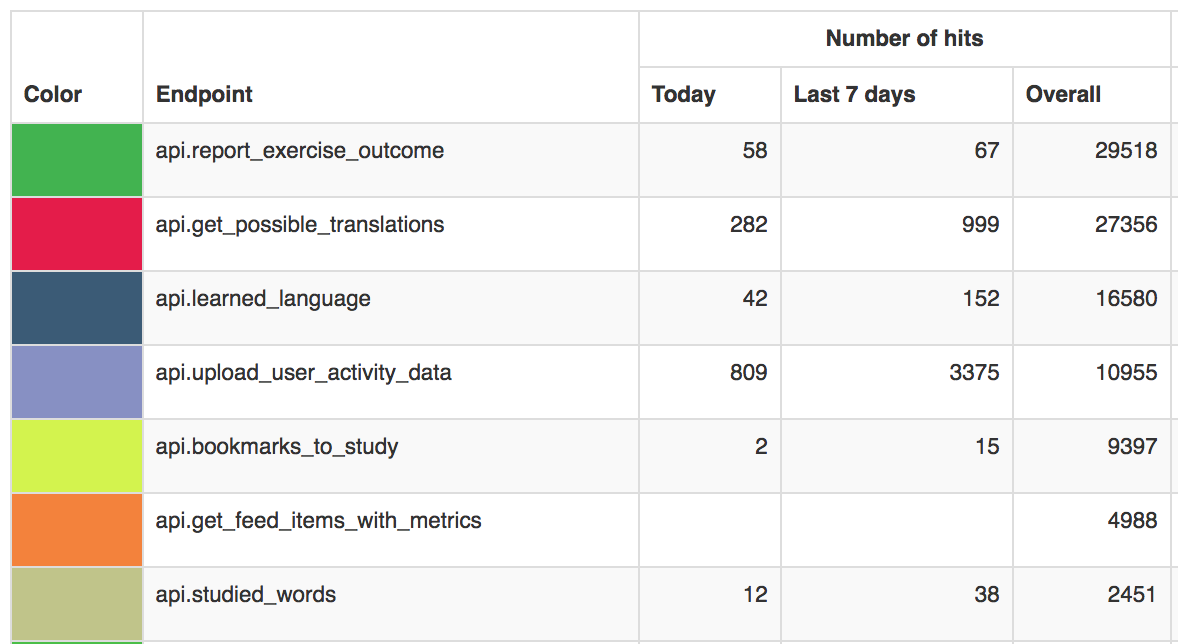
\includegraphics[width=\linewidth]{basicest-utilization}
  \caption{....}
  \label{fig:basicest}
  \end{figure}

This kind of information is already very useful, and can provide the API maintainer with insight into the evolution of their system. By looking at \Fref{fig:basicest}, which presents the top 7 endpoints (for lack of space) one can already see several patterns: 

\begin{itemize}

  \item {\bf Frequent Patterns of System Usage}. The two most used endpoints stand for the two main activities in the system: 

  \begin{itemize}

    \item \epTranslations is an indicator of the amount of foreign language reading the users are doing

    \epOutcome is an indicator of the amount of foreign vocabulary practice the users are doing.

  \end{itemize}

  \item {\bf Sudden Increase of Endpoint Usage}. One endpoint (\epUserActivity) has been disproportionately been used in the last day and last week; much more than before. 

  \item {\bf Possibly Discontinued Endpoint Usage}. One endpoint (\epFeedItems) has not been used in the last 7 days

\end{itemize}

\lesson{Although very useful, it was only after several months of using the system that the client requested the extra columsn for one day and seven days.}

  % \begin{figure}[h!]
  % \centering
  % 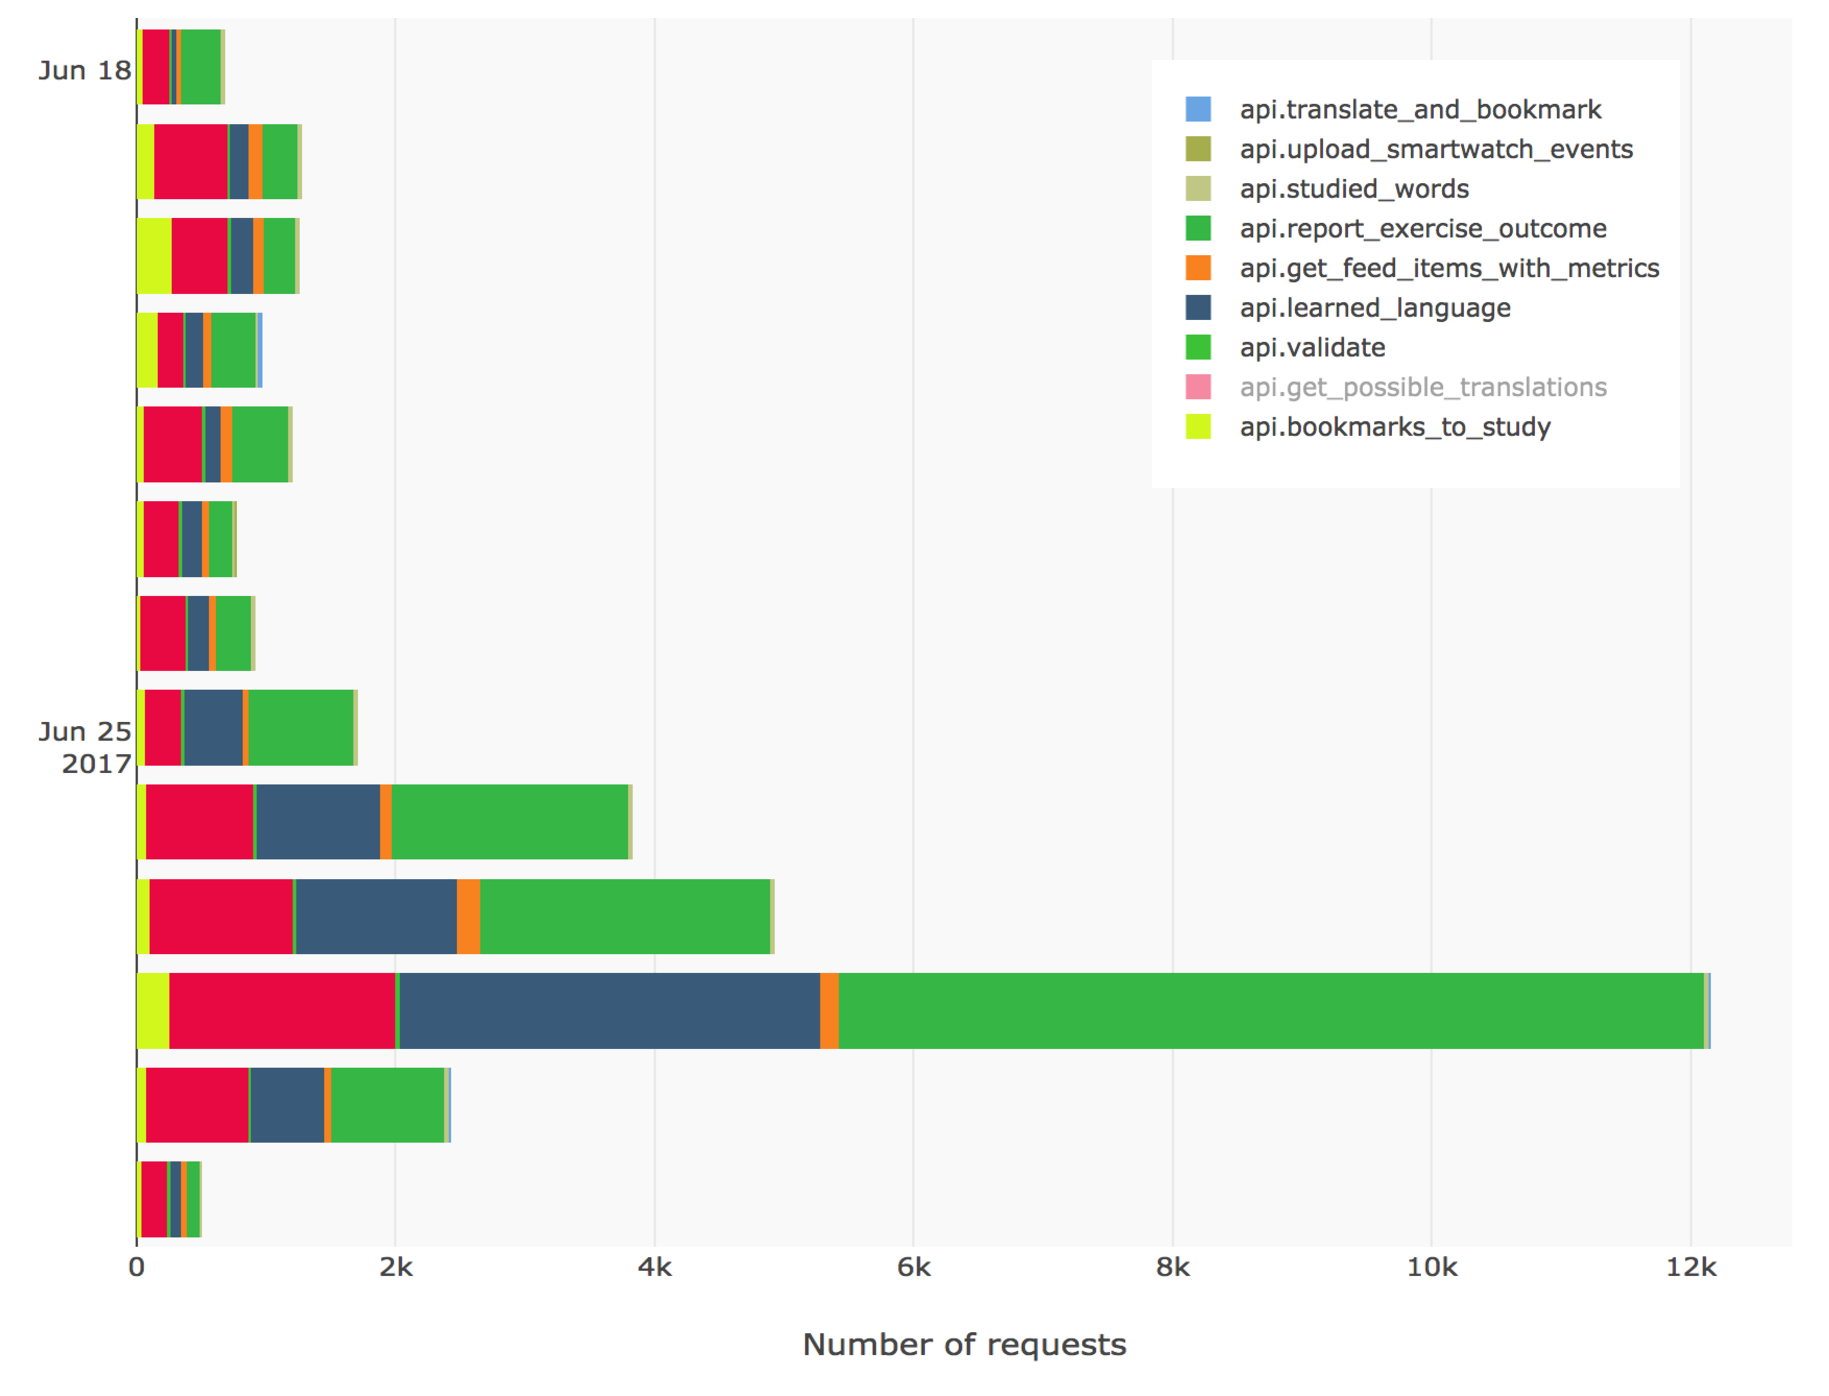
\includegraphics[width=0.5\linewidth]{number_of_requests_}
  % \caption{The number of requests per endpoint per day view shows the overall utilization of the monitored application}
  % \label{fig:aeu}
  % \end{figure}




The table view is limited, and the one day and one week periods are conveniently but arbitrarily selected. For a more detailed evolution of utilization, Figure \ref{fig:aeu} shows the \perspective{Daily Utilization} perspective on endpoint utilization that \tool provides: a stacked bar chart of the number of hits to various endpoints grouped by day\footnote{Endpoint colors are the same in different views}. Figure~\ref{fig:aeu} in particular shows a peak utilization, a day when the API had more than 12.000 hits. 

\begin{figure}[!ht]
\centering
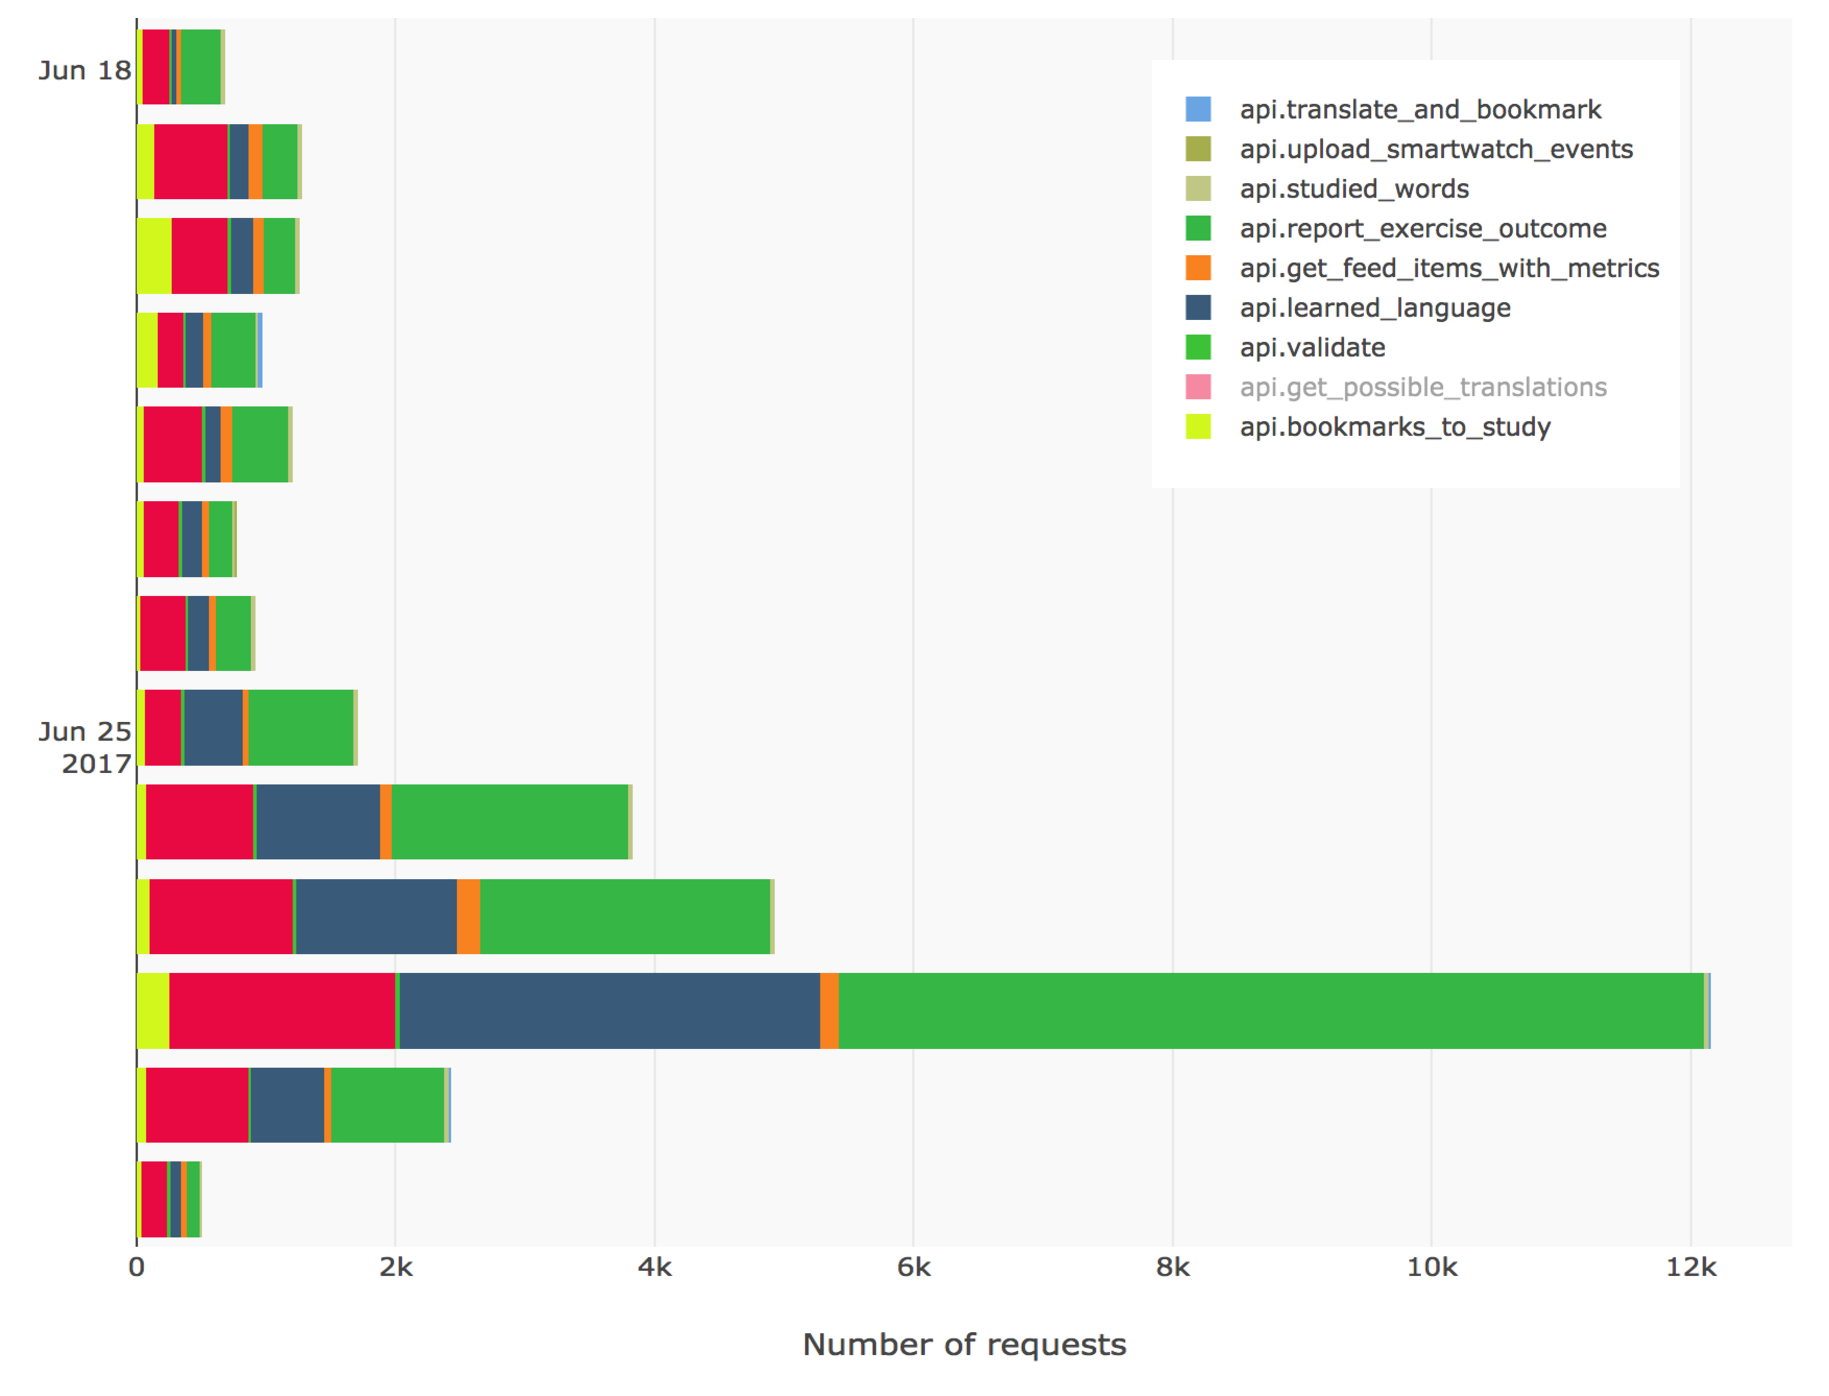
\includegraphics[width=\linewidth]{number_of_requests_}
\caption{Usage patterns become easy to spot in the requests per hour heatmap}
\label{fig:aeu}
\end{figure}


% \begin{figure}[h!]
%   \centering
%   \subfloat[Daily Utilization]{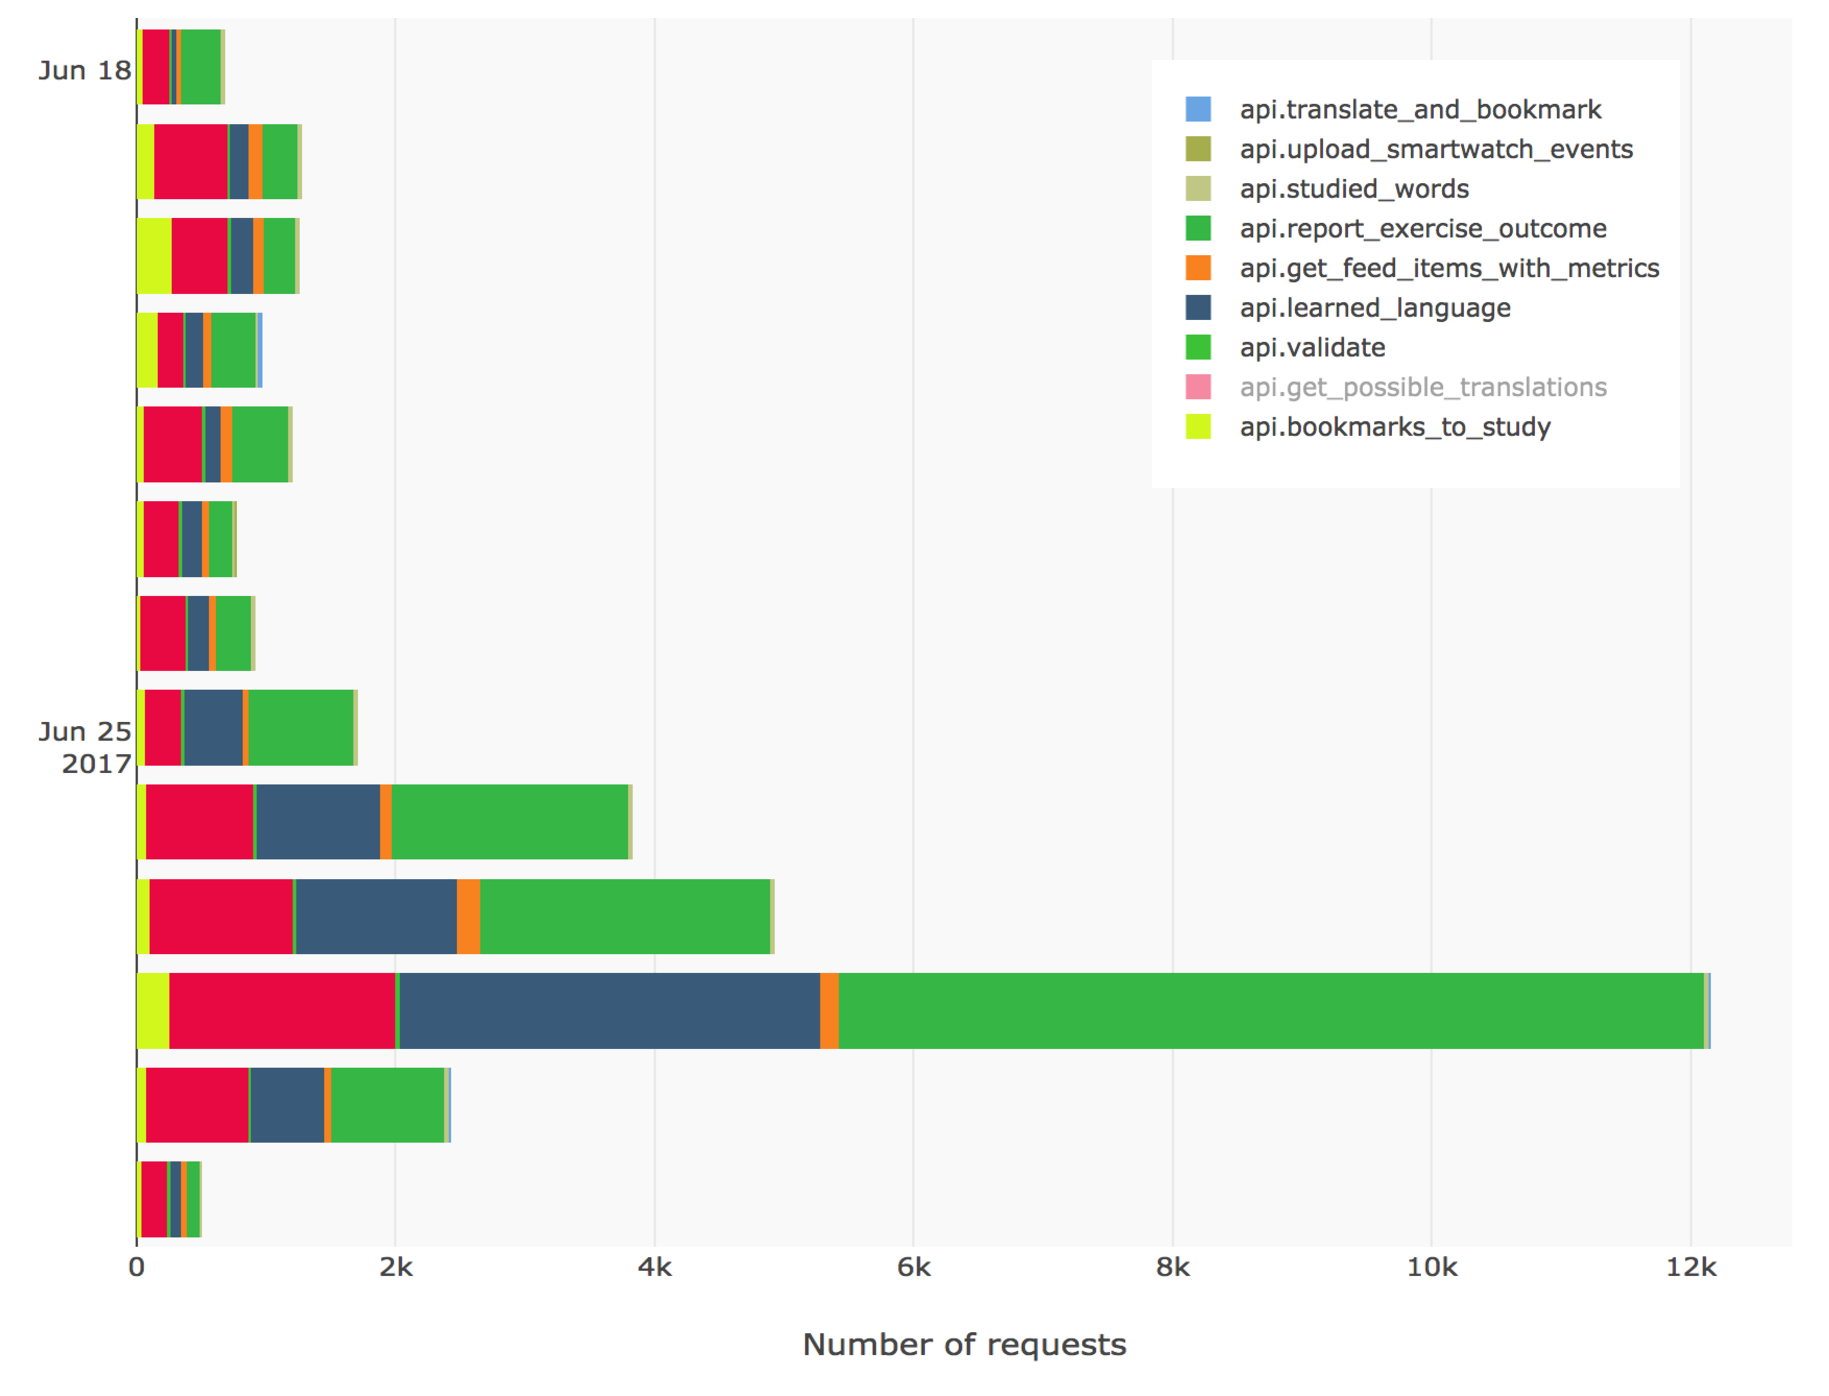
\includegraphics[width=.42\columnwidth]{number_of_requests_}\label{fig:aeu}}
%   \subfloat[Hourly Utilization]{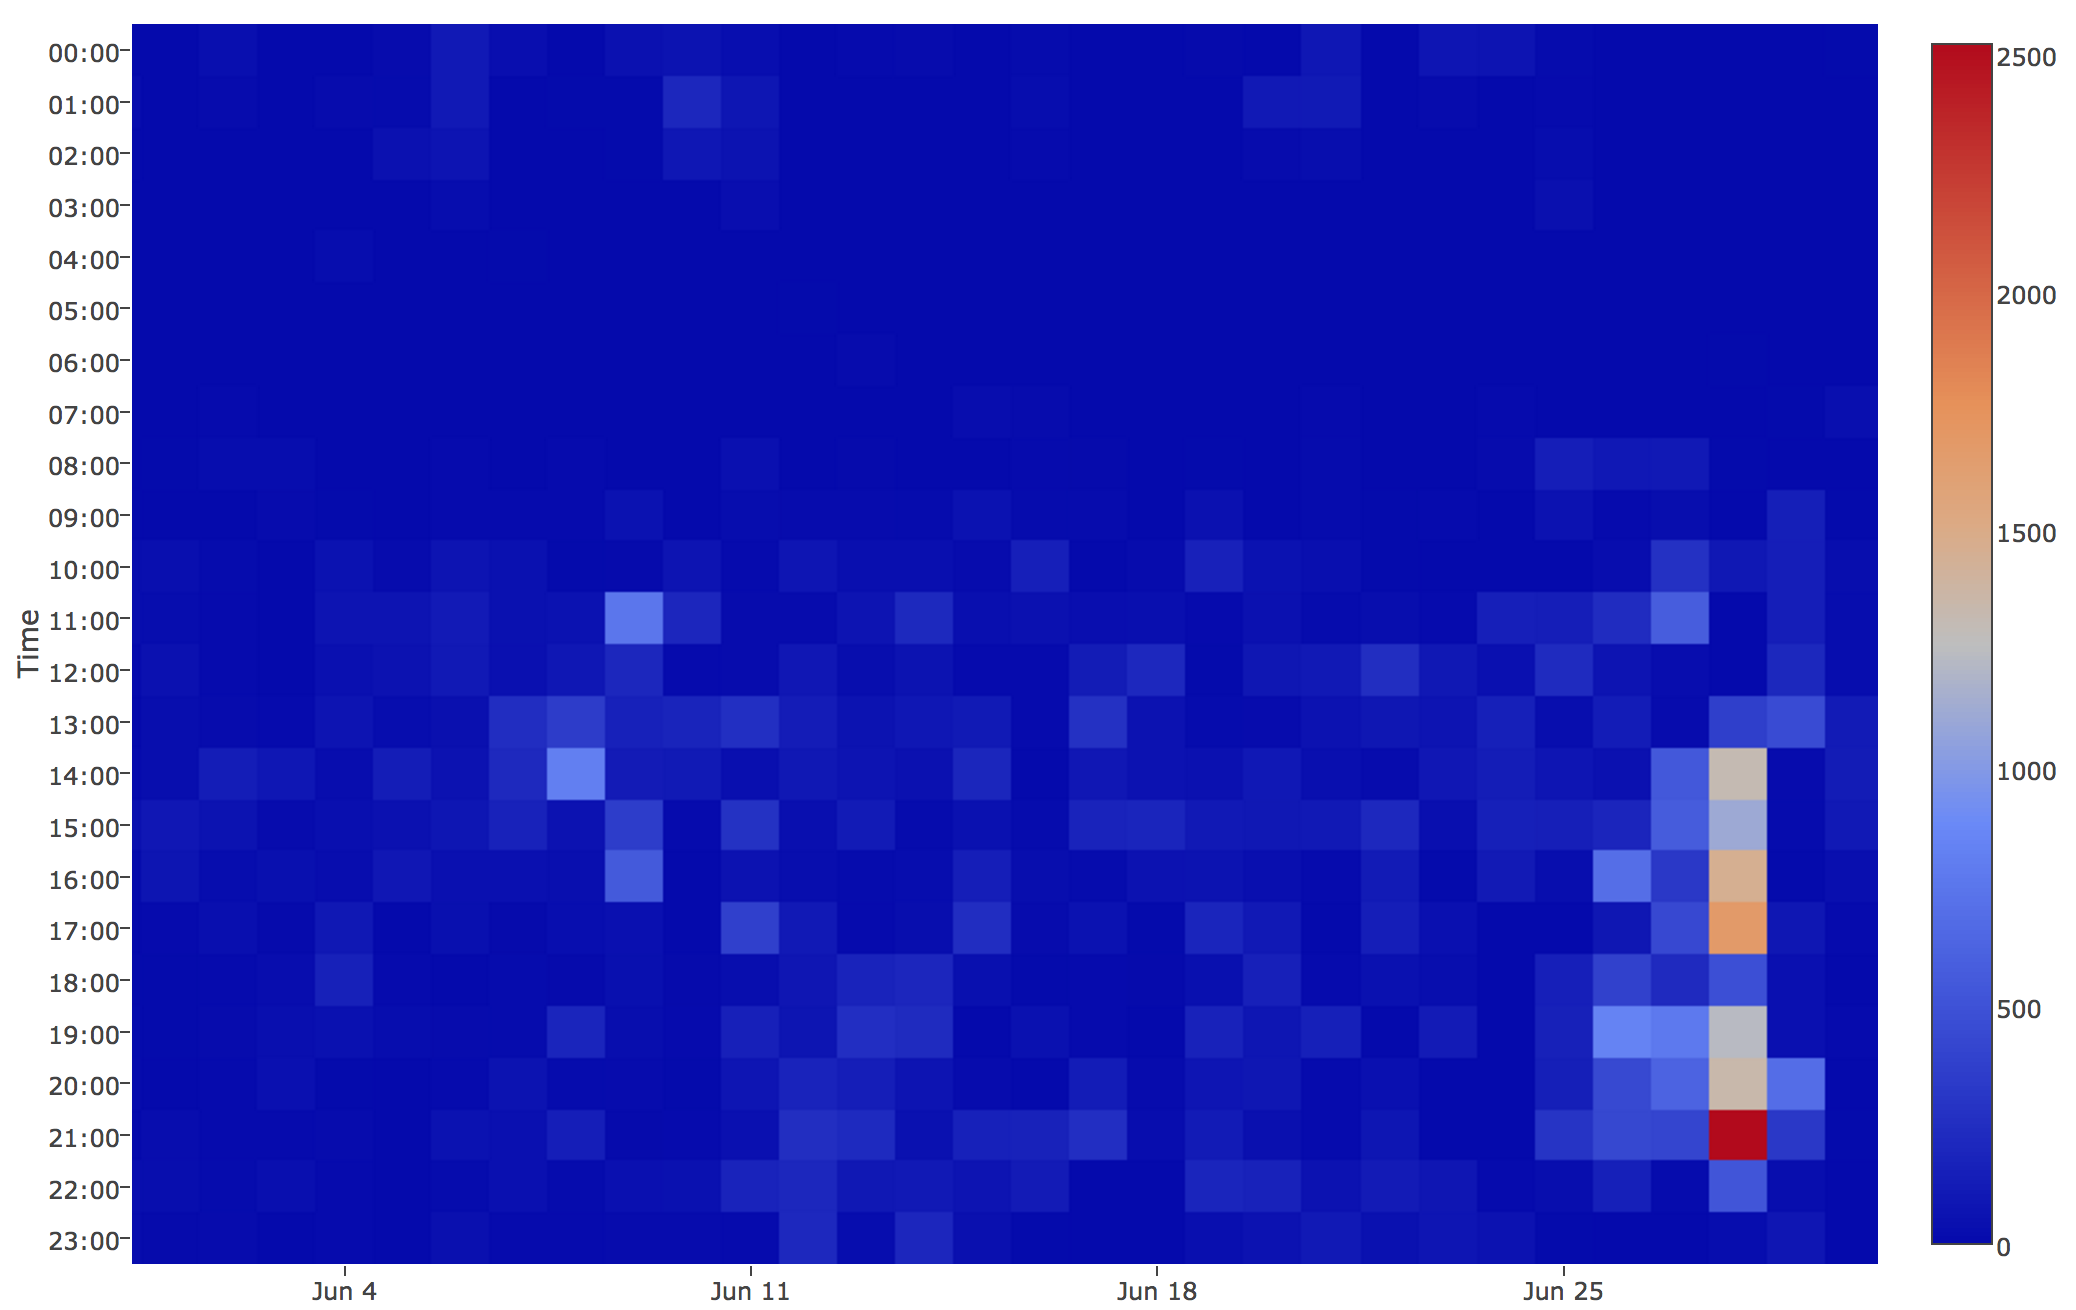
\includegraphics[width=.5\columnwidth]{daily_patterns_}\label{fig:dp}}
%   \caption{Some of the available views\label{fig:views}}
% \end{figure}


% The way users interact with the platform can also be inferred since the endpoints are indicators of different activity types, e.g.: 



% Besides showing the overall utilization, this endpoint provides the maintainer with information relevant for decisions regarding endpoint deprecation --- one of the most elementary ways of {\em understanding the needs of the downstream}\cite{Haen14a}. In our case study, the maintainer realized that one endpoint which they thought was not being used (i.e. \code{words\_to\_study}), contrary to their expectations, was actually being used\footnote{A complementary type of usage information can also be discovered in the view presented in Figure \ref{fig:sep} where seeing that an endpoint is never accessed can increase the confidence of the maintainer that a given endpoint is not used, although it can never be used a proof.}.

% \niceseparator

%   \todo{Add the time series graph and discuss it before the heatmap? We can then sell the heatmap better} 
%   \ml{Not sure about which graph you refer to here V}

Another utilization perspective is the \perspective{Hourly Utilization} in which  the \tool can highlight {\em cyclic patterns of usage per hour of day} by means of a heatmap, as in \Fref{fig:dp}. 


\begin{figure}[!ht]
\centering
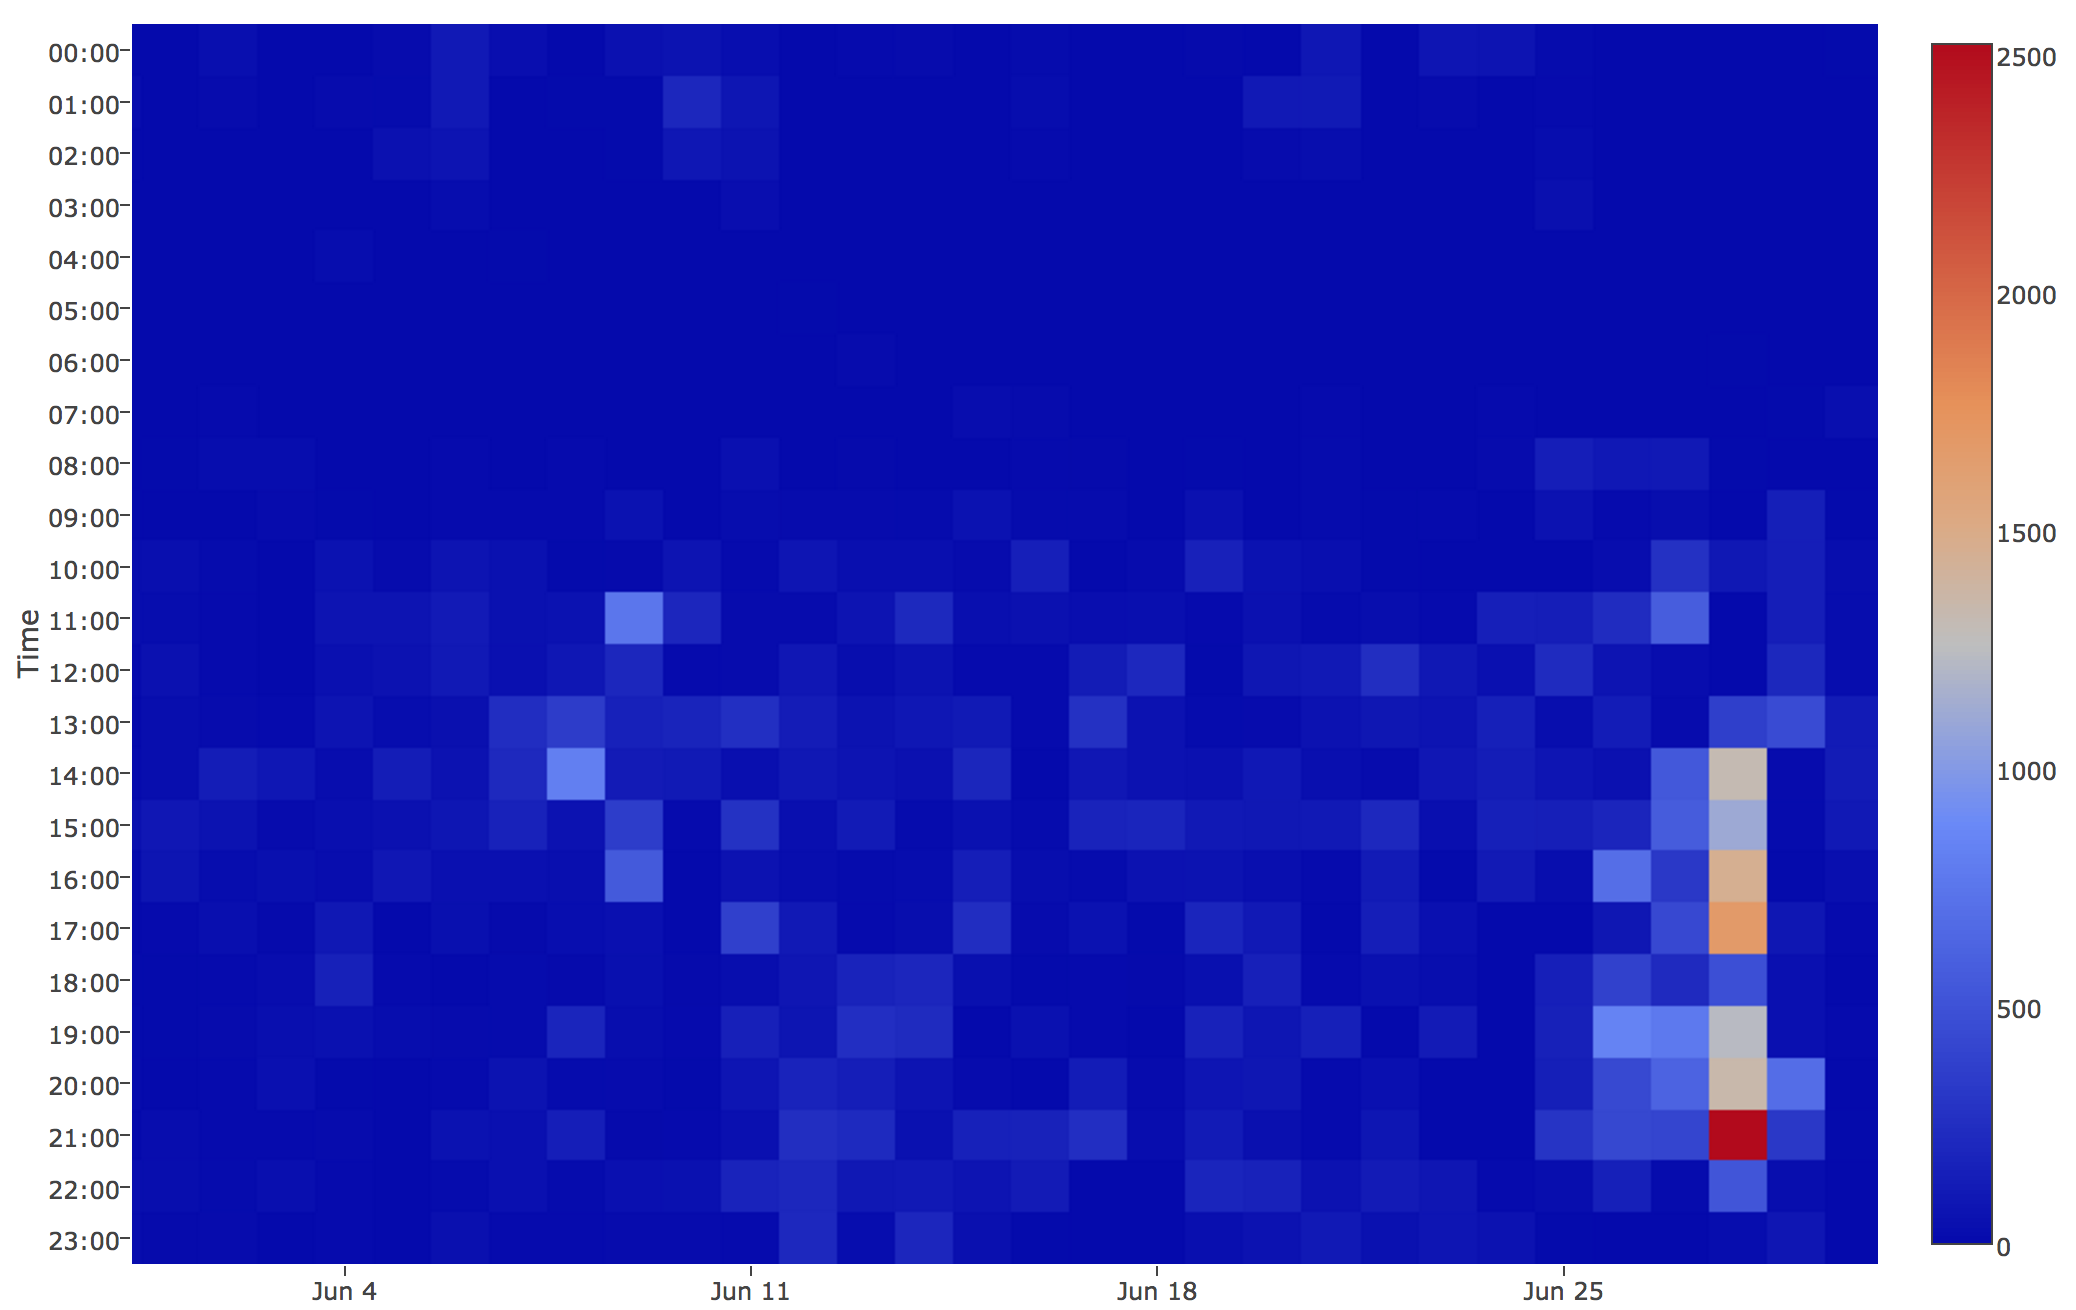
\includegraphics[width=\linewidth]{daily_patterns_}
\caption{Usage patterns become easy to spot in the requests per hour heatmap}
\label{fig:dp}
\end{figure}


Figure \ref{fig:dp} shows the API not being used during the early morning hours, with most of the activity focused around working hours and some light activity during the evening. This is consistent with the fact that the current users are all in the central European timezone. Also, the figure shows that the spike in utilization that was visible also in the previous graph happended in on afternoon/evening.








%!TEX root=restructured.tex

\subsection{Service Performance}
\label{sec:perf}


  The \tool also collects information regarding endpoint performance. The view in \Fref{fig:ep} summarizes the response times for various endpoints by using a box-and-whiskers plot. 

In the Zeeguu case study, one of the slowest endpoints, and one with the highest variability as shown in \Fref{fig:ep} is \epFeedItems: it retrieves a list of recommended articles for a given user. However, since a user can be subscribed to anything from one to three dozen article sources, and since the computation of the difficulty is personalized and it is slow, the variability in time among users is likely to be very large. 


 \begin{figure}[!ht]
   \centering
   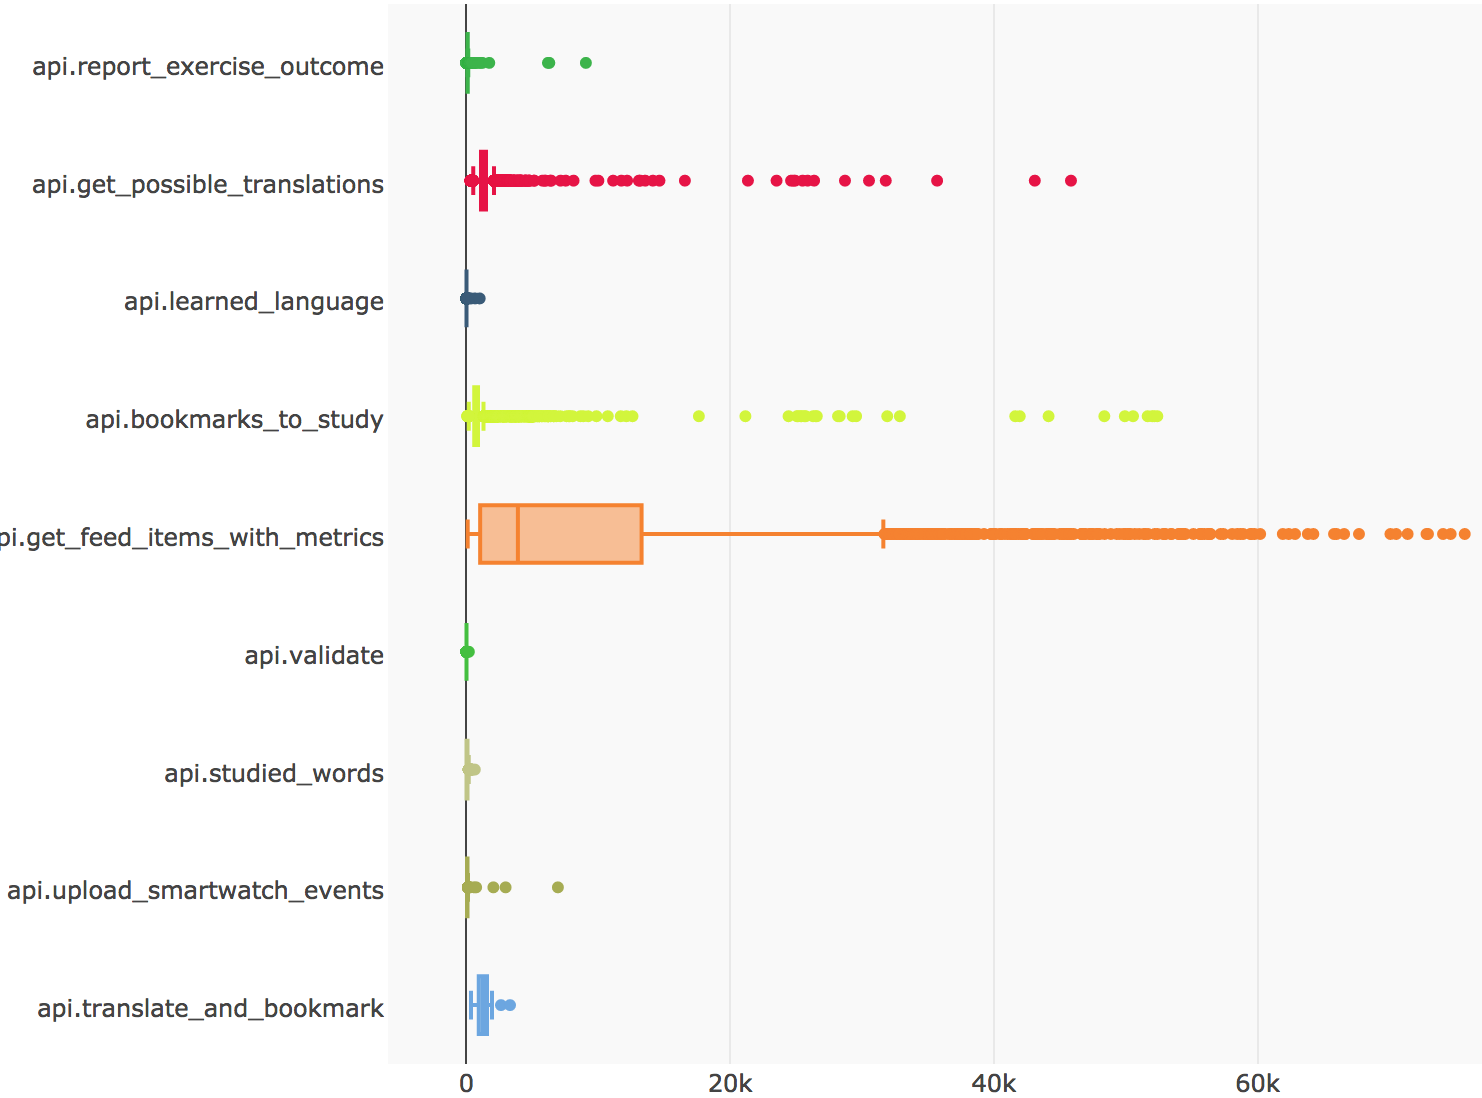
\includegraphics[width=0.95\linewidth]{endpoint_performance_}
   \caption{The response time (in ms) per monitored endpoint view allows for identifying performance variability and balancing issues}
   \label{fig:ep}
 \end{figure}

  From this view it became clear to the maintainer that four of the endpoints had very large variation in performance.   The most critical for the application and consequently the one optimized first was the \epTranslations endpoint which was part of an interactive loop in the reader applications that relied on the Zeeguu API. Moreover, cf. \Fref{fig:aeu} this endpoint is one of the most used in the system.





  \newpage
  \subsection{Performance Insight: Automated outlier detection and monitoring}
  
  When an API is called from within a highly interactive application (as it is the case with the case study in this paper) 
  of particular interest to the API developers are performance {\em outliers}. 

  Indeed, a translation request that takes three times more than expected can seriously decrease the perceived quality of the application. Thus, identifying, collecting all appropriate data, and diagnosing the root causes of such outliers is especially critical in improving the quality of an application. 
  
  % In the context of the RESTful services support by Flask, this means request serving times that deviate from the average to an unexpected degree. 
  
  For this purpose the \tool tracks for every monitored endpoint a {\em running average} response time value\footnote{\ins{For performance reasons, we assume that the response times for the endpoints are normally distributed. Otherwise, more general density distribution information must be collected in real time.}}. When it detects that a given request is an outlier with respect to this past average running value, it triggers the {\em outlier data collection routine} which stores \ins{extra information} about the current execution environment. A configurable threshold with a default value of $2.5$ times the running average response time is used for this purpose. 

  For every detected outlier request, the \tool collects information about the current Python stack trace, CPU load, memory consumption, request parameters, etc. in order to allow the maintainer to investigate the causes of these exceptionally slow response times. In this way it is possible to get \ins{detailed insight into the operation of the application in the extreme cases without unnecessarily burdening it with logging this information for every request}.


  \begin{figure}[h!]
    \centering
    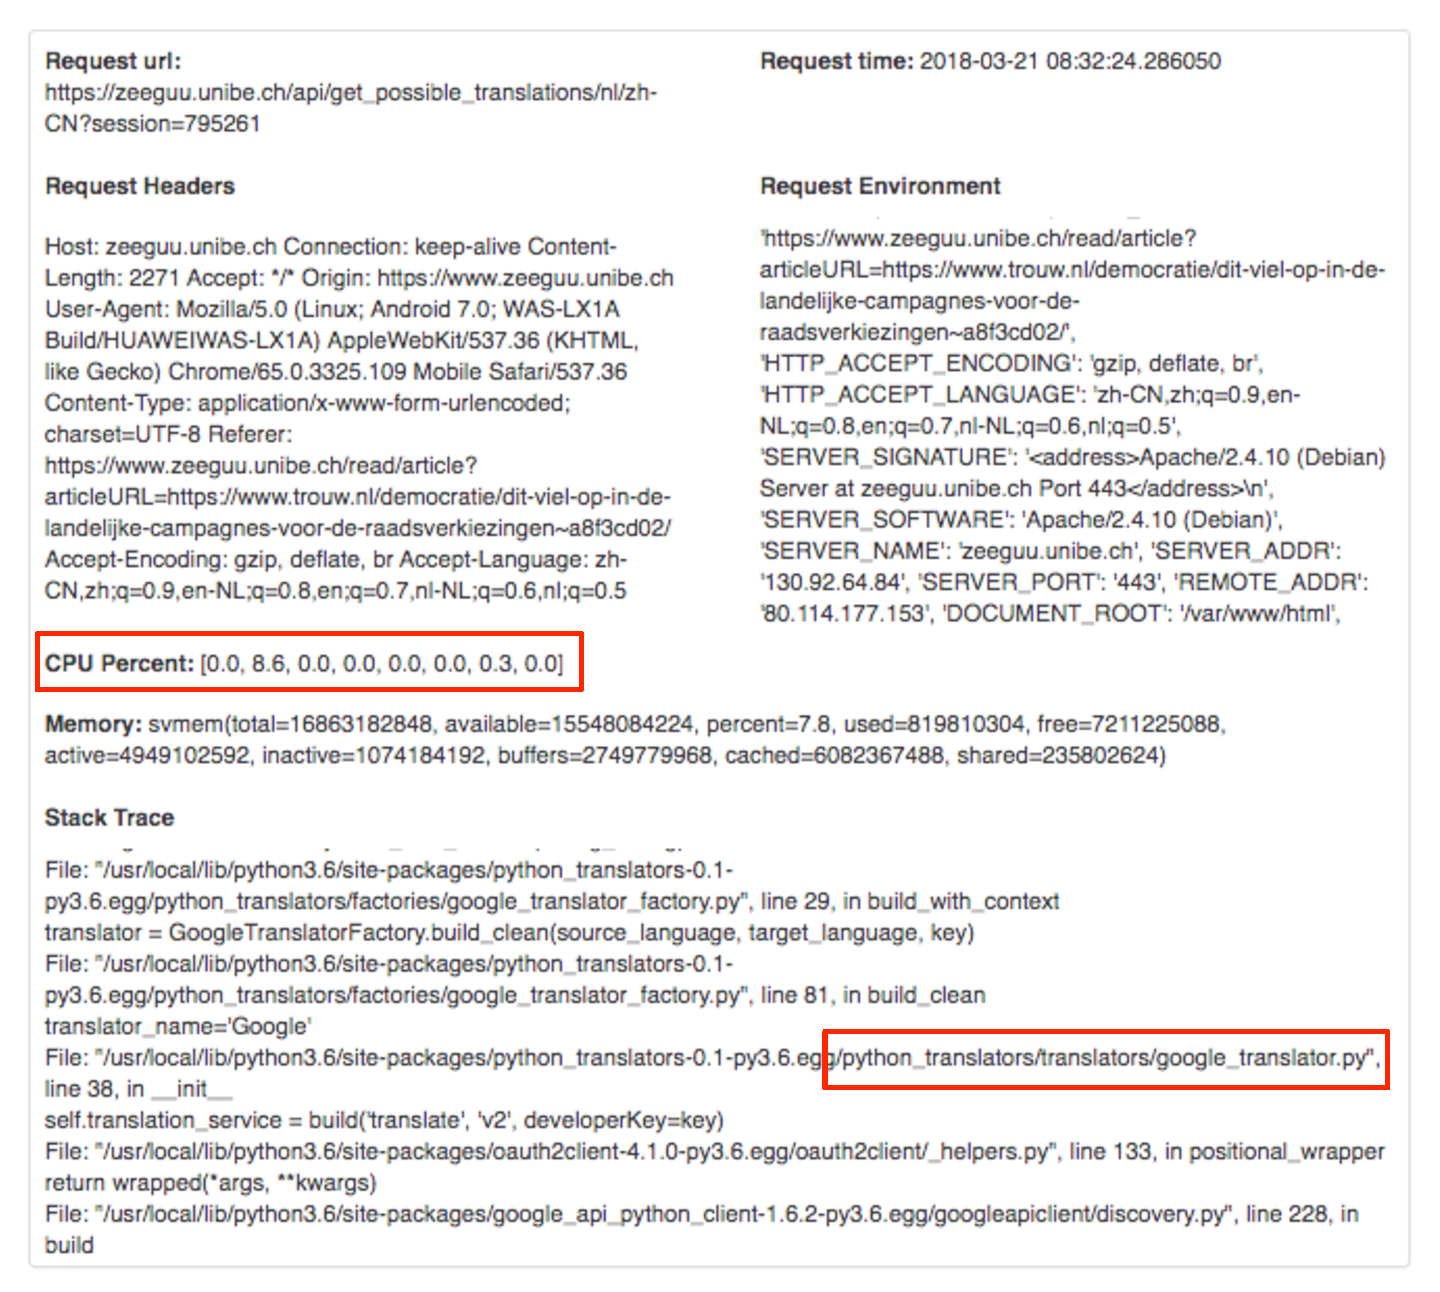
\includegraphics[width=\linewidth]{outlier-annotated}
    \caption{Automatically collected outlier information}
    \label{fig:figure1}
  \end{figure}
  

The bottom panel shows the stack trace. 
In this particular case, it is revealing for the developer to learn that at the time of the stack trace snapshot, the code was in the microsoft\_translator.py: indeed, the system uses as back-end multiple translators, and it has been observed that many of the outliers happen to be waiting in the microsoft translator.

This information has to be corroborated with the observations that neither the memory nor the processor are overloaded at the moment. Thus this functionality in microsoft\_translator is really slow in itself, and this is not a result of the machine being overloaded for example. 









\begin{figure*}[h!]
  \centering
  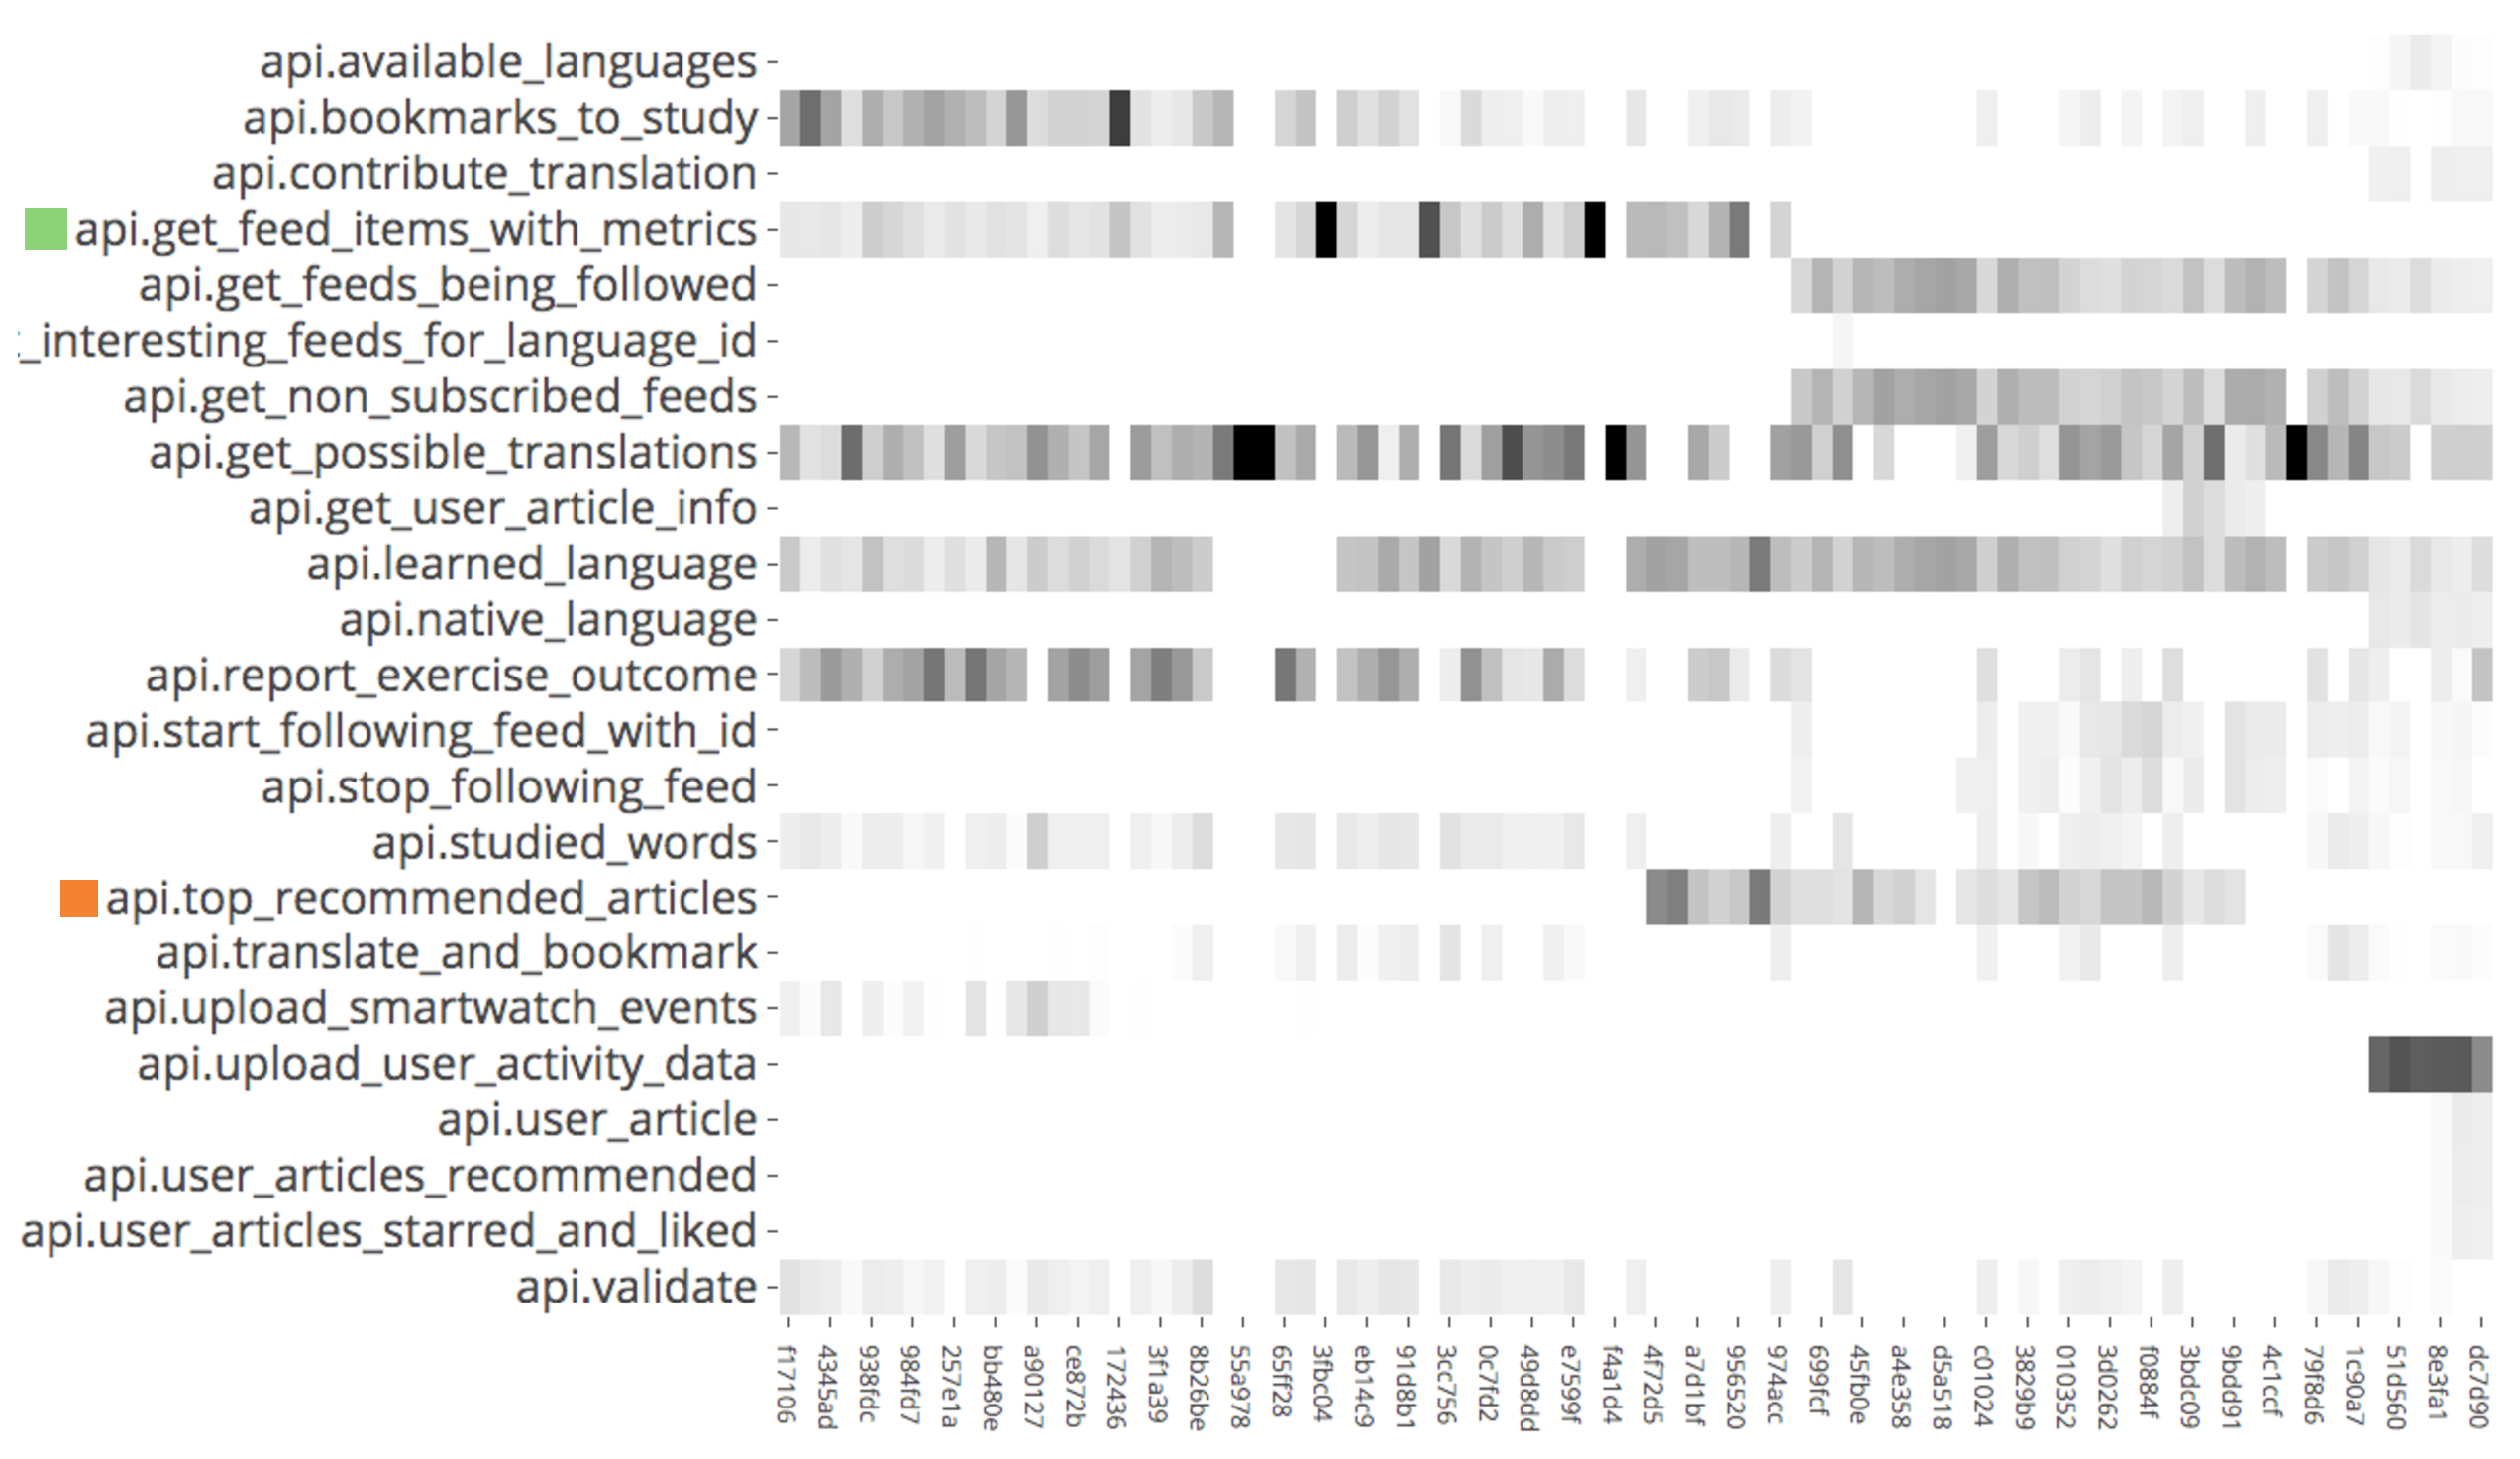
\includegraphics[width=0.9\linewidth]{utilization-evolution}
  \caption{The Evolution of Endpoint Utilization Across System Versions}
  \label{fig:tee}
\end{figure*}



%!TEX root=paper.tex

\section{Identity-Based Grouping of Requests}
\label{sec:grouping}

It is sometimes the case that the utilization and performance of an API must be understood not only per endpoint, but also by grouping the requests by another criterion. Two such examples are: 
\begin{itemize}
	\item When a service has diferent types of users (e.g. the paying vs. the free-for-evaluation ones, or the in-house vs. those in a different organization) the maintainer must understand the performance for the different groups
	\item When the load mix of the users can vary dramatically and the system response time is a function of the individual user load\footnote{E.g. in GMail some users have a few dozen emails while other have tens of thousands: this difference in user loads will eventually induce a difference in the response times for different users} the maintainer must understand the variation of performance with the users (and implicitly the user load).
\end{itemize}

To support narrowing down the analysis to groups of users, or even individual users, the \tool can log together with every request grouping information for that request. The simplest way of achieving this is to take advantage of the architecture of Flask applications in which a global \code{flask.request} is used to retrieve session information which can in turn is normally used to identify the user sending the request. From the user one can obtain the group. 

%\niceseparator

The following code snippet shows how we enabled \tool to enable user-by-user analysis\footnote{If we wanted to group by the user group for example, the code would change slightly by replacing ``user.id'' with ``user.group.id''}: 

\begin{lstlisting}[style=custompython]  
# LOC #2: group requests by user id
dashboard.config.group_by = 'User',
  lambda: Session.find(flask.request).user.id

\end{lstlisting}

The \code{dashboard.config.group\_by} is assigned a tuple with two elements, in which:  

\begin{itemize}
	\item \code{'User'} stands for the name of this particular grouping strategy
	\item \code{lambda: Session.find... } is a callback with no arguments, 
	that makes use of the global \code{flask.request} and extracts from 
	the request the current session, and in turn the user id\footnote{
		Note that every web service or application must have a way of 
		associating a request with a user. In fact, the Session.find(request) 
		was already an existing function in the analyzed system}
\end{itemize}


In Zeeguu, it was decided to further understand the per-user performance of \epFeedItems
~---  an endpoint that retrieves a list of recommended articles for a given user.
It is the endpoint with the slowest response time and highest variability (see \Fref{fig:ep}). 


\begin{figure}[h!]
  \centering
  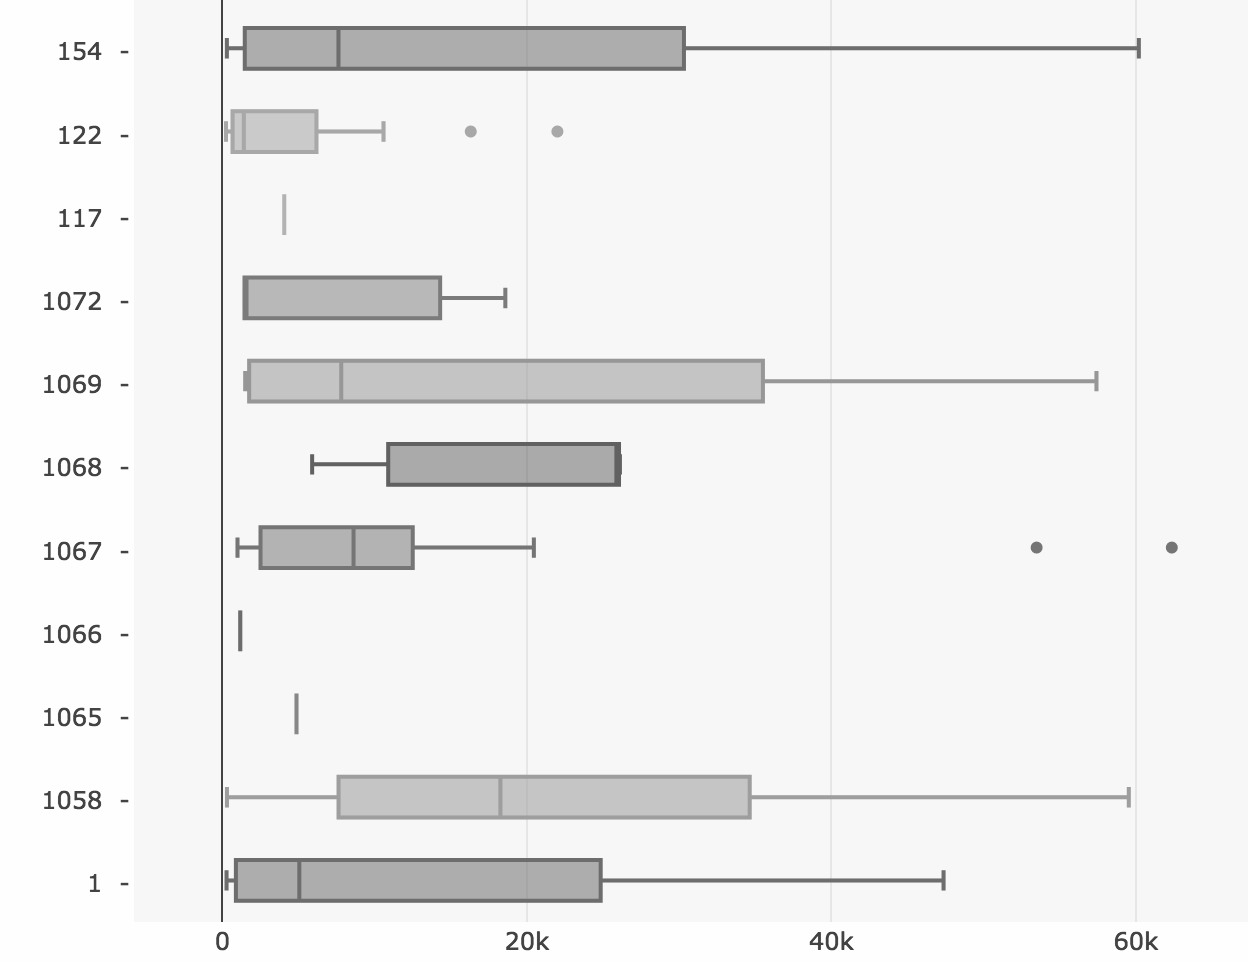
\includegraphics[width=.66\linewidth]{time_per_user}
  \caption{And endpoint with a high variability across users}
  \label{fig:tpu}
\end{figure}


After configuring the \tool as shown earlier, the \perspective{Per-User Endpoint Performance} perspective becomes available to  present the different response times for different users. Figure \ref{fig:tpu} presents a subset of the corresponding view in the \tool. The figure shows that the response times for this endpoint varied considerably for different users with some extreme cases where a user has to wait a full minute until their recommended articles were shown. 

The reason for this behavior is that a user can be subscribed to anything from one to three dozen 
article sources and for each of the sources the system computed the personalized difficulty 
of each article at every request. After seeing the two perspectives presented in Figures \ref{fig:ep} and \ref{fig:tpu}, the \zee maintainer refactored the architecture of the system to move this difficult computation out of the interactive loop.








%!TEX root=paper.tex
  
  \section{Version-Aware Monitoring}
  
  The Stack Overflow Developer Survey from 2018 revealed the fact that 88.4\% of professional developers use git for version control. 
  Given that versioning using git is the main way in which the source code of services evolves, it is natural to monitor their progress also across versions. 

  Version control in \tool can be supported in two ways,
  the developer explicitly states the current version, 
  or the current version is automatically detected based
  on some version control system. 


  % However, with the current configuration of the tool, it would be impossible for the maintainer to see the improvements resulting from the optimization. 

  If assume that the code that they run is deployed using .git, then with an extra line of configuration they can allow \tool to find the git\footnote{\url{https://git-scm.com/}} folder of the deployed service and automatically detect the version of the project that is running: 
    
\begin{lstlisting}[style=custompython]

# LOC #3: provide the dashboard with 
# information on where to find the 
# git information 
dashboard.config.git = 'path/to/.git'
  
      
\end{lstlisting}  
 
  If the \tool can automatically detect the current version of the project by reading the .git configuration as soon as the API is started and can then group measurements by version\footnote{Alternatively, the maintainer can add version identifiers manually for the web application through a configuration file if the system does not use git.}. 


  

  \subsection*{Evolving Utilization}

  \Fref{fig:mv-util} shows the \perspective{Multi-Version API Utilization} perspective which presents the utilization of the tracked endpoints across versions. Because the different versions might be deployed for very different periods of time, at the intersection of an endpoint and a version the chart does not plot the absolute utilization of that endpoint in that version but rather the percentage of all the API calls that go to that endpoint. Otherwise a version that is deployed for many weeks would make all those deployed for several days invisible.


    \begin{figure}[h!]
      \centering
      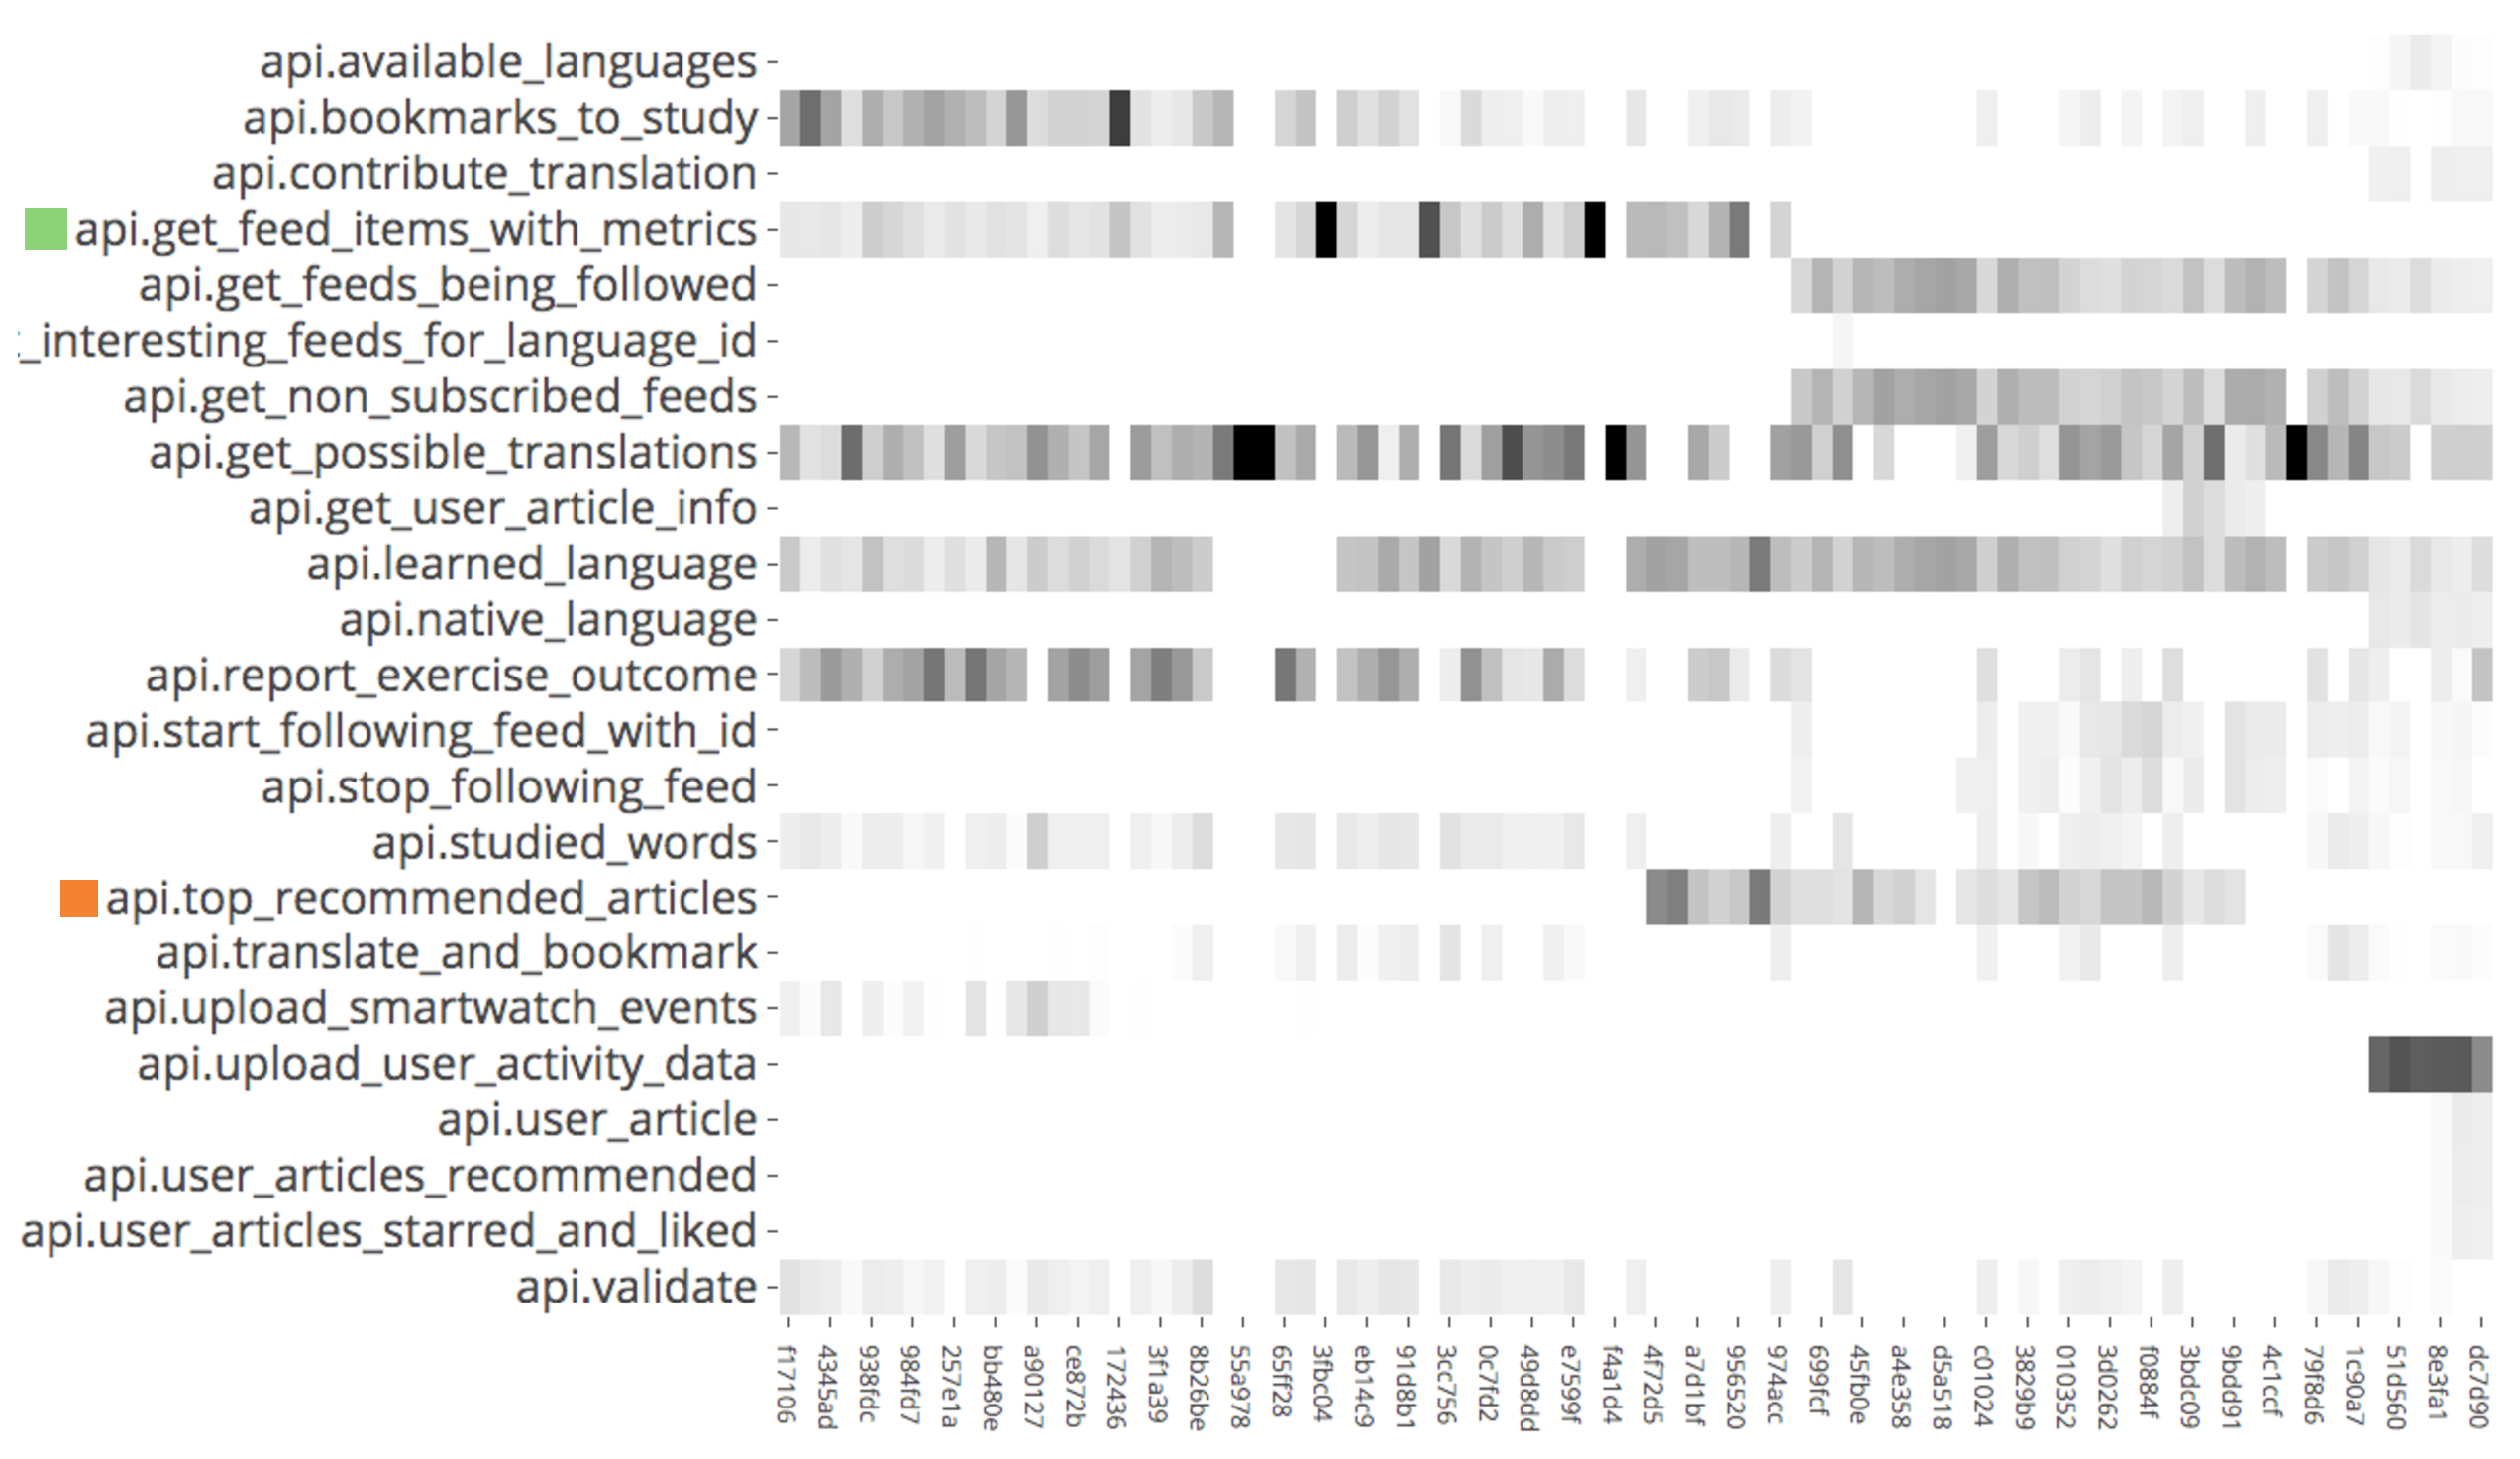
\includegraphics[width=0.9\linewidth]{utilization-evolution}
      \caption{The Evolution of All the API Endpoints Utilization Across System Versions}
      \label{fig:mv-util}
    \end{figure}

  With this view, several patterns are visible:
  \begin{itemize}
    
    \item \epFeedItems is discontinued a little bit after \epTopArticles is being introduced

  \end{itemize}


  \subsection*{Evolving Performance}

    \Fref{fig:tee} is a zoomed-in version of such a view for \epTranslationsColor with versions increasing from top to bottom

    \begin{figure}[h!]
      \centering
      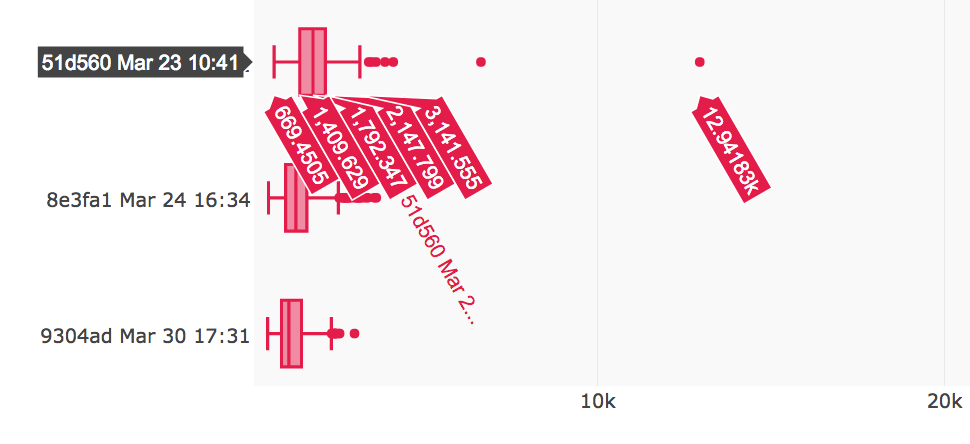
\includegraphics[width=0.9\linewidth]{translation_endpoint_evolution_}
      \caption{The Performance Evolution of the \epTranslations endpoint}
      \label{fig:tee}
    \end{figure}


  This view confirms that the performance of the translation endpoint improved in the recent versions: the median of the last three versions is constantly moving towards the left, and progresses from 1.4 seconds (in the top-most box plot in \Fref{fig:tee}) to 0.8 in the latest version (bottom-most box plot).


\subsection*{Evolving Grouped Performance}
  The limitation of the previous view is that it does not present the information also on a per version basis. To address this, a different visual perspective entitled \perspective{User-Focused Multi-Version Endpoint Performance} can be defined. Figure \ref{fig:tuv} presents such a perspective by mapping the average execution time for a given user (lines) and given version (columns) on the area of the corresponding circle. 

\begin{figure}[h!]
  \centering
  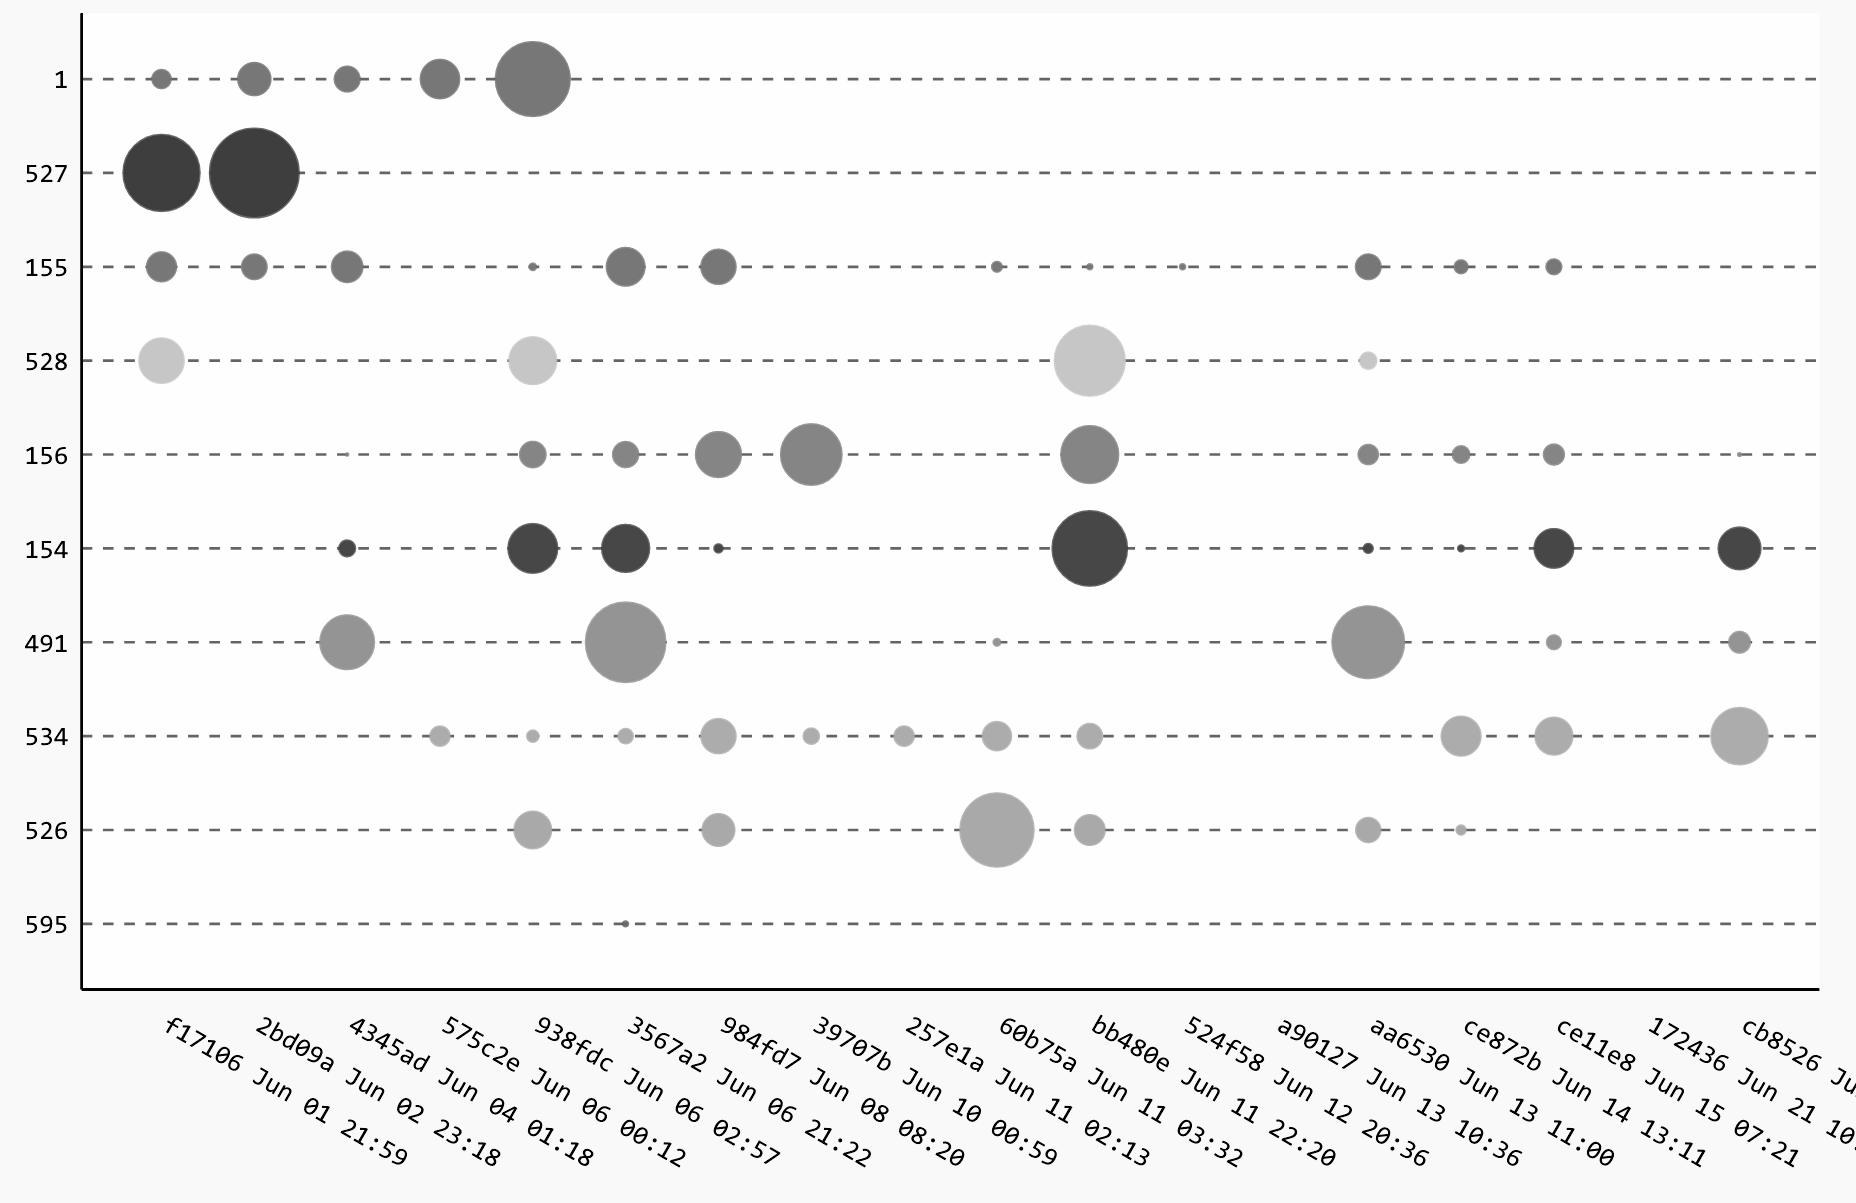
\includegraphics[width=0.77\linewidth]{time_per_user_per_version}
  \caption{This perspective shows that the evolution of response times for individual users (horizontal lines) across versions (the x-axis) for a given endpoint}
  \label{fig:tuv}
\end{figure}


The colors represent users. The figure shows average performance varying  across users and versions with no clear trend: this is probably because varying user workload (i.e. number of sources to which the user is registered) is the reason for the variation in response times. \ins{one can see that for user 1 performance degrades over the versions. Given that for other users the performance does not degrade in the same way, it is probable that the problem might lay elsewhere: the server was overloaded or the endpoint is ``algorithmically slower''.}


  


%!TEX root=paper.tex

  \begin{figure*}[h!]
  \centering
  \subfloat[The reported response time (in ms) per deployed version in the observation period]{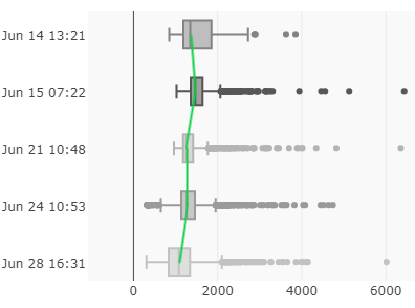
\includegraphics[width=.6\columnwidth]{response_per_version_trunced_trend}}
  \quad
  \subfloat[The measured response time (in ms) using integration with Travis]{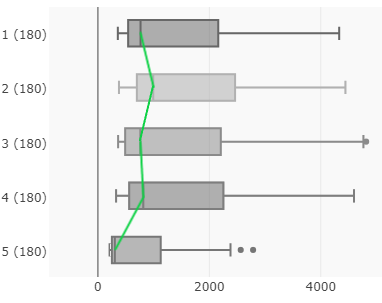
\includegraphics[width=.56\columnwidth]{travis_builds_no_outliers_trend}}
  \caption{Comparison of the response times per endpoint: actual production system versus preemptive monitoring data}
  \label{fig:preemptive}
\end{figure*}


  \section{Preemptive monitoring}

  \ins{INTRO - LINKING WITH PREVIOUS PARAGRAPH: the previous evolutionary view crucial for 
  understanding the impact of software evolution on performance.
  However, just by observing this one can't be sure whether 
  performance changes because of the code or because of the payload.}
  
  \todo{the following might need a bit of rewrite}
  
  The concept of {\em preemptive monitoring} of the application performance by means of instrumenting integration unit testing as the synthetic load is similar to the idea of augmenting service monitoring with online testing~\cite{metzger2010proactive}, i.e.~testing service-based applications by using dedicated test input in parallel to its normal use and operation. The difference is that we take advantage of the capability of the CI framework (i.e. Travis in this case) to create an emulated ``live'' environment for integration testing purposes, and use unit testing as the dedicated test input in order to measure performance. 
  

      \begin{figure}[h!]
        \centering
        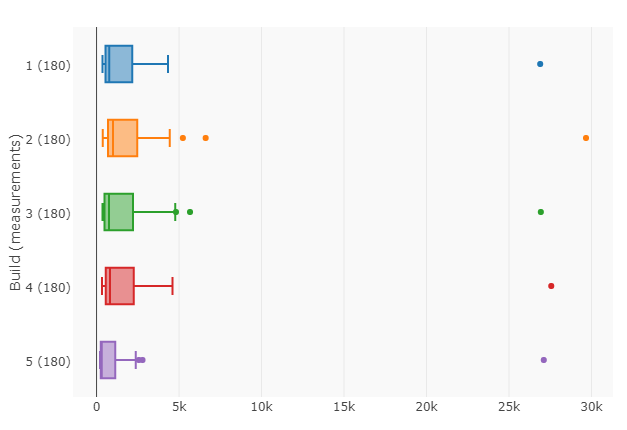
\includegraphics[width=0.7\columnwidth]{travis_builds}
        \caption{Response times in 5 consequent Travis builds in the \zee case study}
        \label{fig:builds}
      \end{figure}



  For example, \Fref{fig:builds} is a screenshot from the dashboard showing the measured response times for 5 consequent builds, with 180 iterations of the unit tests executed in total across all endpoints. The outliers on the right of the figure are due to initial requests \ins{which must wait for a boot-up phase of the API}.  



  
  While this integration testing environment is different from the actual production deployment one, and the load used is purely synthetic, as will show in Section~\ref{sec:evaluation}, it can actually be used successfully as an early performance indicator for the application developer. \ins{Although predicting the performance of the application would require advanced statistical work, it can be succesfully used as an advanced warning system for the overall performance trend for given endpoints}.  


  \paragraph{Integration with Travis}
  \ml{added new section... also, this has to be moved after introducing the pre-emptive monitoring since it's about running tests. switched the order}
  

  \ins{The pre-emptive monitoring system} can be configured to work together with Continuous Integration (CI) frameworks like Travis\footnote{\url{https://travis-ci.org/}} that deal with automated integration testing.
  The developer needs to define the unit test folder of the project, the URL that Travis should use for reporting its results, and the number of iterations for each unit test should be executed in order to generate a load for the application. 
  
  Each time a new build is created through Travis, the \tool automatically detects all available unit tests defined by the application developer and iterates through each one of them the number of times predefined by the developer while monitoring the response times for each request. The resulting measurements are persisted in a separate part of the tool database so as not to contaminate the ``live'' monitoring data. Beyond seeing the results of each Travis build in the \tool, this feature also allows for preemptive monitoring of the application, as we discuss in the following.    

  \ins{Besides functioning as an early warning system for performance, tracking the evolving performance of API tests serves a second purpose. To function as an anchor when the developer analyzes performance degradations. For example, when a developer sees that a given endpoint has become less performant after in a newly deployed version, they are able to investigate whether the performance degradation is visible also with the synthetic load. This would correspond to a performance degradation which is due to ``algorithmic performance degradation''. If on the other hand, the performance of the tests does not change between versions, the developer might conclude that the performance degradation could be due to the workload on the machines, or maybe to the workload mix of the users}
  
  %By these means, an application developer can use unit tests as synthetic loads for driving the performance monitoring of the application before it reaches the production phase.  As we will discuss further in Section~\ref{sec:testing}, this feature is integral in enabling preemptive performance monitoring of the application.  
  

\todo{here goes the discussion about our forecasting capabilities}



\begin{table}[h]
  \begin{tabular}{lll}
    \toprule
    Iteration & \bfseries Live (median) & \bfseries Travis (median)\\
    \midrule
    1 & 1349.41 & 764.87\\ 
    2 & 1466.13 & 992.87\\
    3 & 1256.65 & 760.87\\
    4 & 1266.42 & 813.89\\
    5 & 1080.68 & 303.4\\
    \bottomrule
  \end{tabular}
\end{table}

Pearson correlation $r(3)=.93, p=.02$




    \begin{figure*}[ht!]
      \centering
      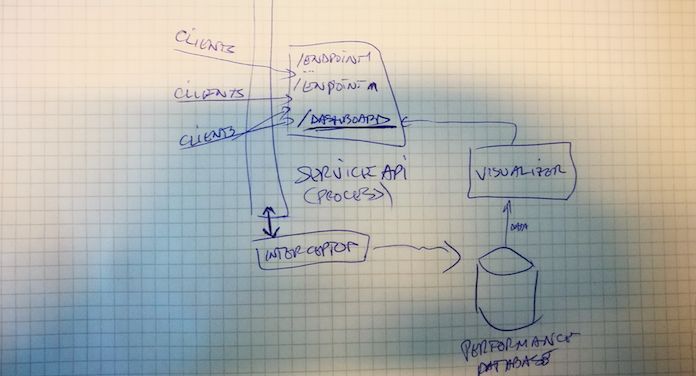
\includegraphics[width=0.8\linewidth]{interceptor}
      \caption{The first thing that needs to be done, is to decorate the application object with an INTERCEPTOR}
      \label{fig:sep}
    \end{figure*}

\newpage


%!TEX root=paper.tex
  
\newpage
\section{Overhead of the \tool}
\label{sec:overhead}

To measure the performance overhead of the \tool, we have implemented an automated benchmarking system. It is open source and available online and can be tested by the reader. The benchmark downloads the latest version of the \zee API and installs it in a Docker container. Then it calls several selected endpoints for 500 times each, tracking the response times. The endpoints are called in three different configurations: 

	\begin{enumerate}
		\item With no dashboard installed
		\item With the dashboard enabled but with the outlier detection deactivated
		\item With the dashboard enabled and the outlier treshold set to zero, thus effectively treating every request {\em like it were an outlier}\footnote{This forces all the requests to be treated as outliers, and thus provides insight into this situation, which otherwise would be hard to generate}.
	\end{enumerate}



\Fref{fig:bench} and Table \ref{tab:benchmark} present with violin plots and respectively descriptive statistics the distribution of times resulting from running the benchmark for three different endpoints on a quad-core machine, with Intel Core i5-4590 processor, @ 3.30GHz, 8G of RAM and 240GB SSD disk drive.


\begin{figure}[h!]
	\centering
	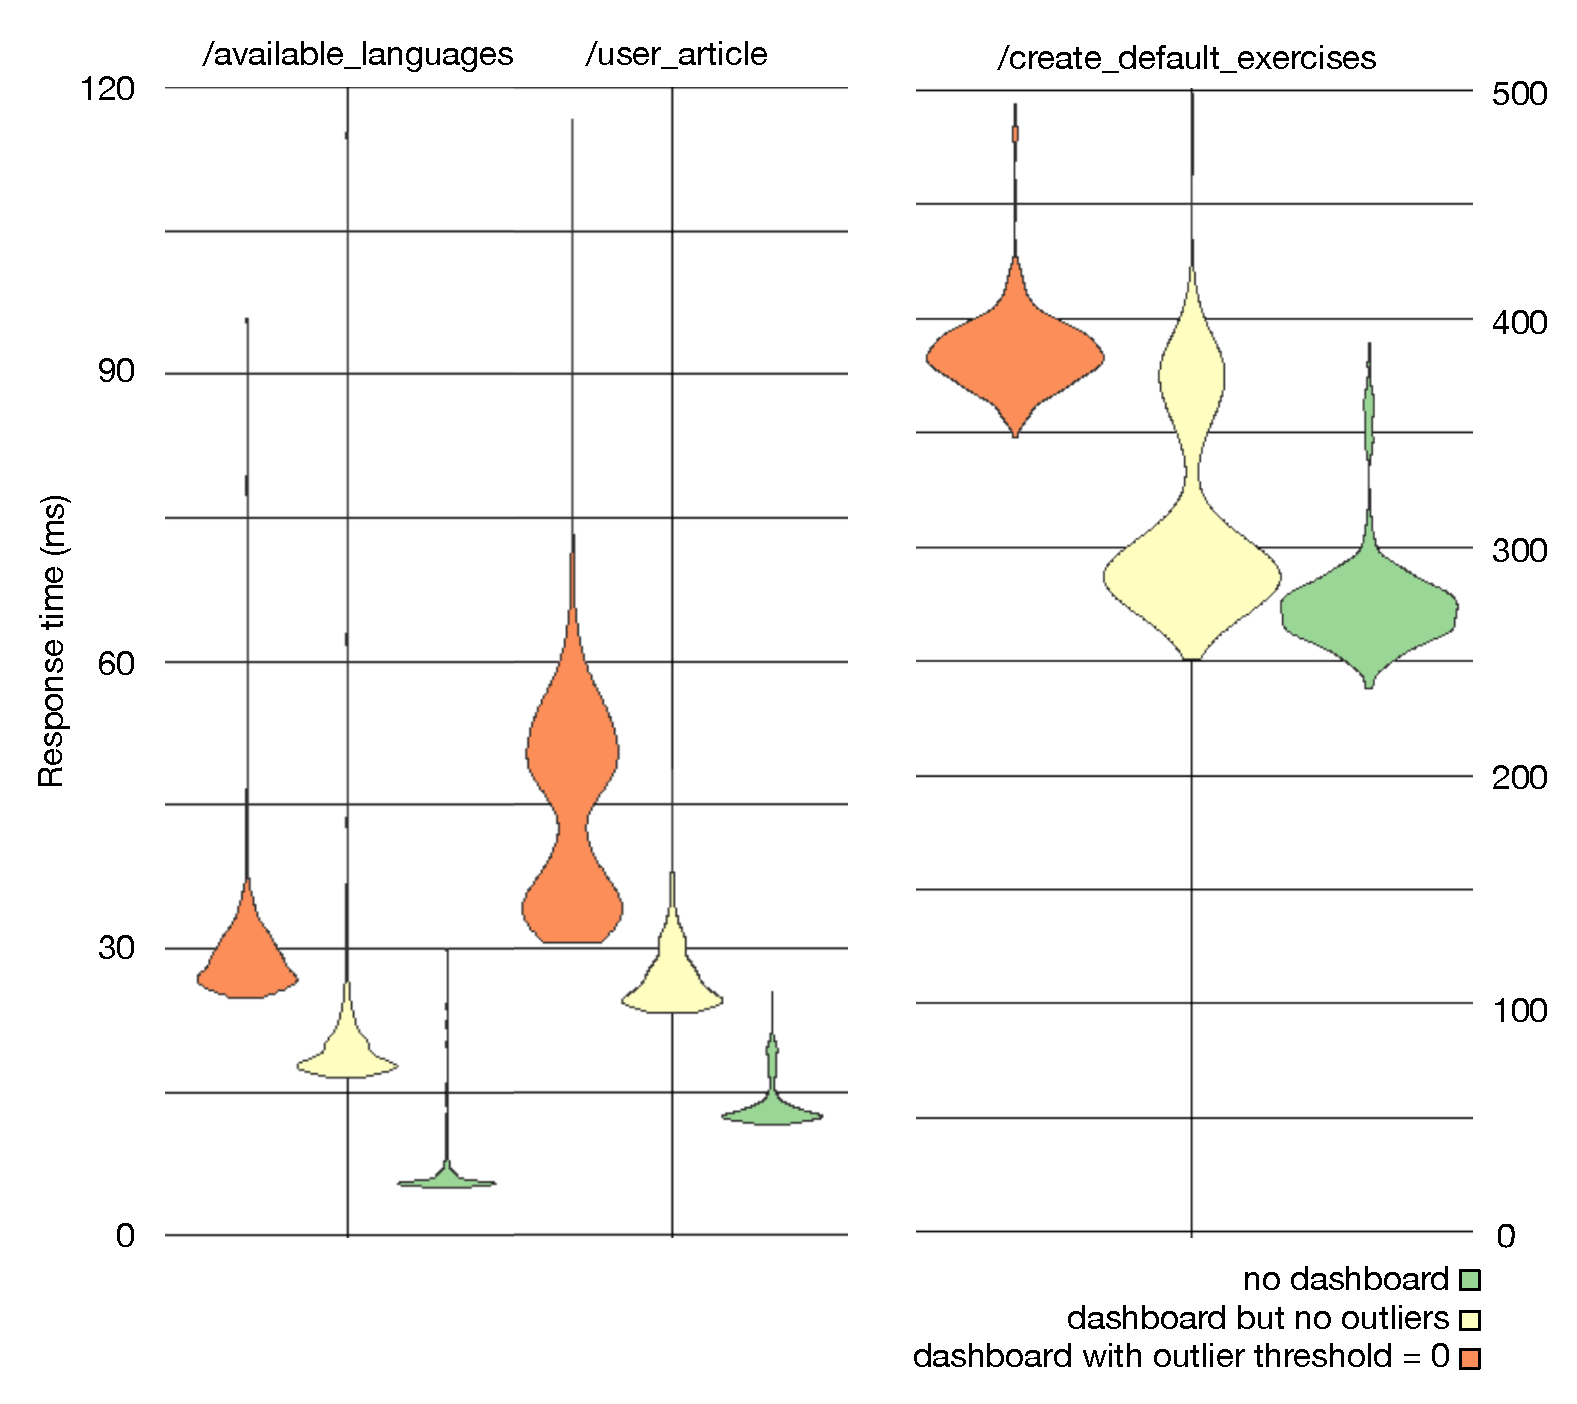
\includegraphics[width=\linewidth]{benchmark2.pdf}
	\caption{The distribution of response times when calling the three endpoints for 500 times in three conditions: no dashboard, dashboard but no outliers, dashboard and every request treated as an outlier}
	\label{fig:bench}
\end{figure}


%!TEX root=paper.tex

\newcommand{\yes}{\checkmark}

\begin{table}[tb]
	
	\centering

	\begin{tabular}{rllrr}
		\toprule
		\bfseries Endpoint & \bfseries Dash. & \bfseries All Out. & \bfseries Mean (ms) & \bfseries SD (ms) \\

		\midrule

	         available\_languages  &    &	    &   6.3 &  2.3 \\ 
	         available\_languages  &  \yes &    &  19.9 &  5.6 \\ 
	         available\_languages  &  \yes &  \yes &  29.4 &  5.4 \\ \\ 

	                user\_article  &    &	    &  13.9 &  2.6 \\
	                user\_article  &  \yes &    &  26.9 &  3.2 \\
	                user\_article  &  \yes &  \yes &  44.8 & 10.0 \\ \\

	    create\_default\_ex...     &    &	    &  276.0 & 22.4 \\ 
	    create\_default\_ex...     &  \yes &    & 313.6 & 43.2 \\
	    create\_default\_ex...     &  \yes &  \yes & 385.3 & 16.9 \\
	
		\bottomrule

	\end{tabular}
	\caption{Response times for three endpoints run 500 times in three different conditions each. Dash. = with dashboard. All Out. = every call being considered an outlier}
	\label{tab:benchmark}

\end{table}




	The three endpoints that are tested fall in two categories of complexity: 
	\begin{itemize}
		\item The two fast ones, are very simple. 
		The first returns a list of language codes which are defined in the code, so it does not touch the DB. The second does a simple read from the database. 
		\item The slower endpoint, does several complex writes to the database, so this is why it is much slower. However, in our case study, about half of the measured endpoints were at least as slow as this one, so its response time is representative.
	\end{itemize}

	The data shows that the dashboard (without outliers) introduces for the faster endpoints an overhead of ~14ms and for the slower endpoint an overhead of ~40ms. 
	In the case of an outlier, the overhead is doubled, so the design decision of only collecting the extra information only for outliers is valid.
	Depending on the application these numbers might be acceptable or this might be too much. In the case of the \zee case study, the maintainers find this acceptable. 



  

% %!TEX root=paper.tex

    \begin{figure*}[ht!]
      \centering
      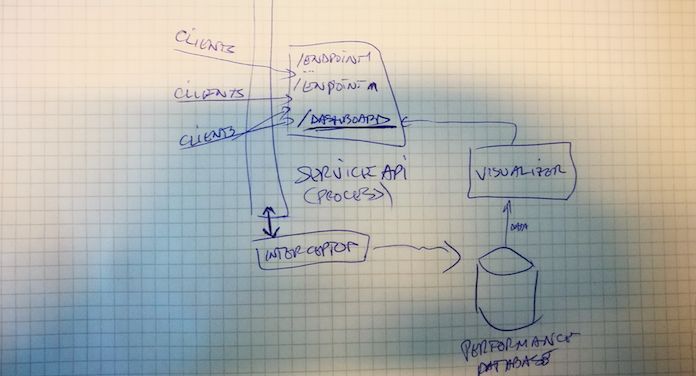
\includegraphics[width=0.8\linewidth]{interceptor}
      \caption{The first thing that needs to be done, is to decorate the application object with an INTERCEPTOR}
      \label{fig:sep}
    \end{figure*}


\section{Architecture}

REMEMBER THE GOAL: Our main goal with the \tool issues to allow the integration of the dashboard with an API with minimal effort.

The fact that the \tool itself is being developed in Python using Flask makes binding to the services of a to-be monitored application developed with the same technologies easy and intuitive. However, by writing different backends that do the measurement and monitoring, the frontend can be reused. 

The viewpoints we showed are only a subset of all the viewpoints of the \tool. In practice, the tool provides other perspectives as long as they are a combination of: 

\begin{itemize}
  \item Cardinality: one endpoint vs multiple
  \item Objective: utilization vs. performance (response time)
  \item Evolution Axis: time vs. versions
  \item Grouping: Grouped (e.g. by user) vs. All
\end{itemize}






\ins{The first important question that such a 
service monitoring system should provide is 
information about what endpoints are being
used and by whom}. 

TODO: Find references, arguments, related work
that provide more details about why understanding
who uses endpoints, and which are used are important.

This is clearly the case in static analysis (see paper
by haenni and lungu...) but should even more be the
case in APIs.




  \newpage


  % This used to be in the first section... 
  % Maybe it fits better localized here: 
  Data collected by the wrappers are persisted in a local database. The SQLAlchemy Object Relational Mapper\footnote{\url{https://www.sqlalchemy.org/}} on top of SQLite\footnote{\url{https://www.sqlite.org/}} is used for this purpose.

TODO: TALK ABOUT THE METAMODEL...


    \begin{figure}[ht!]
      \centering
        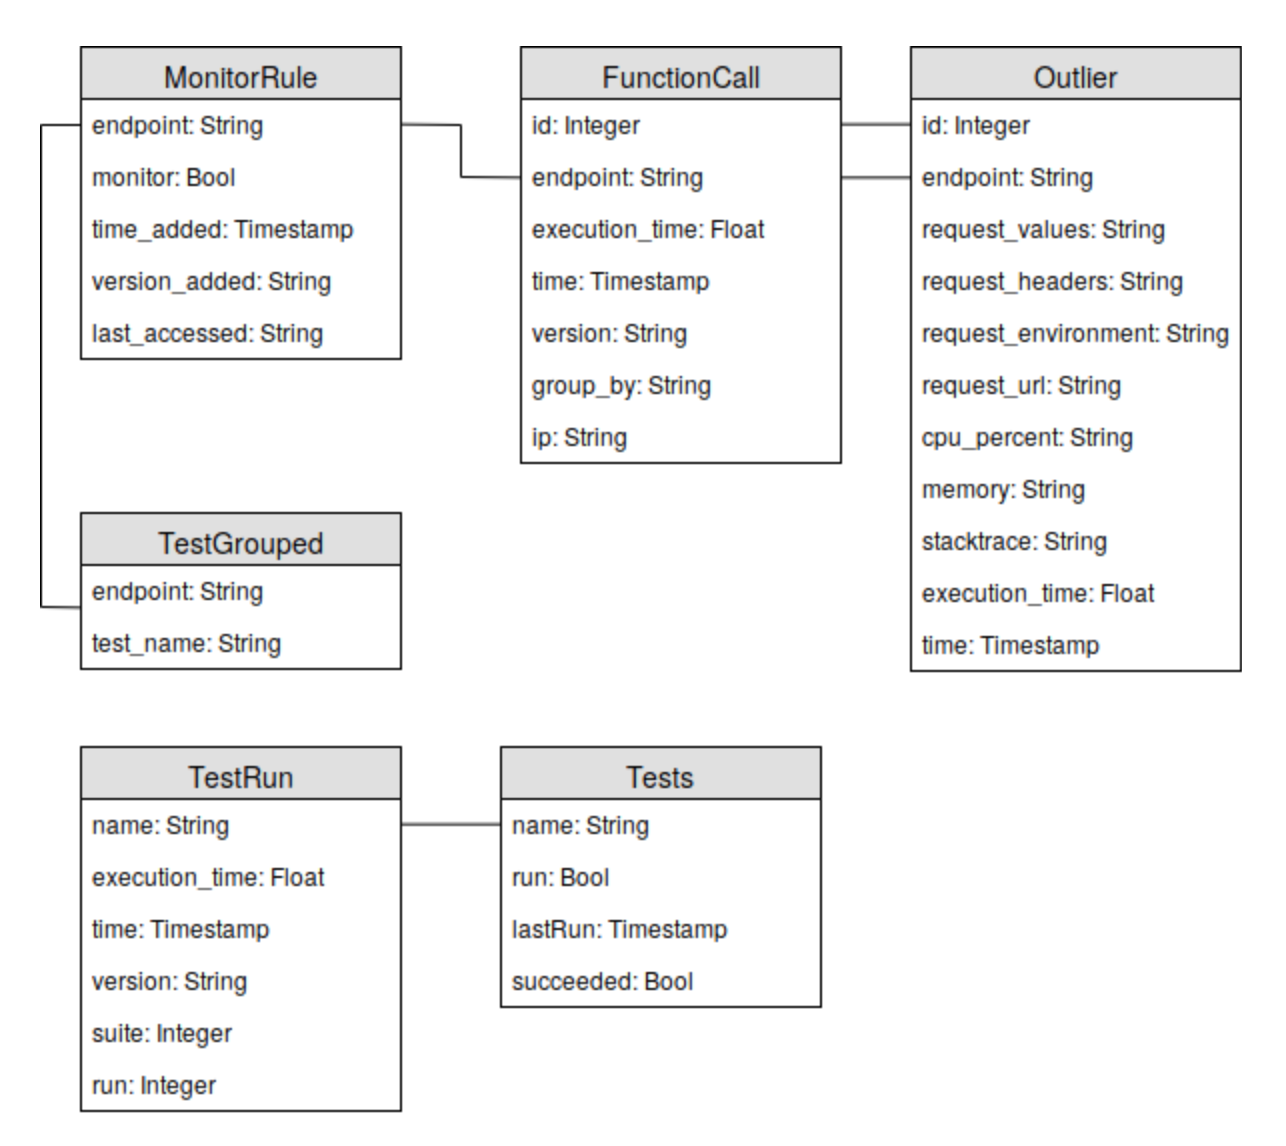
\includegraphics[width=0.8\linewidth]{db_schema}
        \caption{The model that supports the views presented in this paper}
        \label{fig:sep}
    \end{figure}

  As discussed in the introductory section, in previous work~\cite{vogel2017low} we introduced \tool, a drop-in Python library that allows developers to monitor their Flask-based Python web applications with minimal effort.
%
  The \tool is implemented for Python 3.6 and is available on the Python Package Index repository\footnote{\url{https://pypi.python.org/pypi/flask-monitoring-dashboard/1.8}} from where it can be installed by running \install from the command line. 
%  
  The source code of the \tool is published under a permissive MIT license and is available on GitHub\footnote{\url{https://github.com/flask-dashboard}}.
  
  




%!TEX root=paper.tex

\section{Discussion}

-   \ins{We can do this minimal configuration for any technology. We showed here how to do it for Python and Flask because they are some of the most popular web development technologies at the moment.}

-   The fact that the \tool itself is being developed in Python using Flask makes binding to the services of a to-be monitored application developed with the same technologies easy and intuitive. However, by writing different backends that do the measurement and monitoring, the frontend can be reused.

- A Special Type of Outlier: Exceptions. TODO: probably something for the journal extension ...
  statistics about which endpoints fail most often might be useful too.
  same information as the outlier maybe?

- time as measured in days and commits are two sides of the same coin. 

- currently the system supports only one grouping. this need not be so, and there are many scenarios where one could envision multiple groupins in parallel.

- threats to the validity of the constant-load performance testing. performance regressions? 
- the endpoint where the unit-testing results can be uploaded is prone to being tampered with by Bob who would want to upload junk information to mess up with the dashboard. to solve this, a UUID can also be added that is generated by the server, and thus prevents anybody else but the rightful owner of the dashboard 

- user management. although not explained in the paper, the dashboard also comes with a user management system. and two classes of users. admins and guests.

- Although predicting the performance of the application would require advanced statistical work, it can be succesfully used as an advanced warning system for the overall performance trend for given endpoints.



\todo{use this subsection to discuss limitations (from the previous evaluation section) and add the need to be able to handle the horizontal scaling of the application; remove sectioning and summarize briefly limitations that have already been discussed in the VISSOFT paper/move material to other sections; consider renaming as limitations or something similar}

  \subsection{Distributed System Monitoring}
  \todo{To think about}
  Supporting situations where the API is deployed across multiple containers for example.


  \subsubsection{Automatically Monitoring System Evolution}

  The main goal of the \tool design was to allow analytics to be collected and insight to be gained by making the smallest possible changes to a running API. %To allow the collection of evolutionary information 
%
  This technique assumes that the web application code which is the target of the monitoring is deployed using \git in the following way: 

  \begin{enumerate}
    \item The deployment engineer pulls the latest version of the code from the integration server; this will result in a new commit being pointed at by the HEAD pointer. %than previously
    \item The deployment engineer restarts the new version of the service. At this point, the \tool detects that a new HEAD is present in the local code base and consequently starts associating all the new data points with this new commit\footnote{The \tool detects the current version of the analyzed system the first time it is attached to the application object, and thus, assumes that the Flask application is restarted when a new version is deployed. This is in tune with the current version of Flask, but if the web server will support dynamic updates in the future, this might have to be taken into account}.
  \end{enumerate}

  The advantage of this approach is the need for minimal configuration effort, as discussed in the presentation of the tool. The disadvantage is that it will consider on equal ground the smallest of commits, even one that modifies a comment, and the shortest lived of commits, e.g.~a commit which was active only for a half an hour before a new version with a bug fix was deployed, with major and minor releases of the software. %as a distinct way of grouping the data points. 
  A mechanism to control which versions are important for monitoring purposes is therefore required to be added.
%
  A further possible extension point here is supporting other version control systems (e.g. Mercurial). However, this is a straightforward extension.

  \subsubsection{NEW: API Renames}
  \ml{just an idea}


    The history would normally be lost in the case of an API rename. (also known as the {\em provenance issue} in source code evolution analysis)
    In theory we could infer that an API was renamed if it is not to be found anymore, and another one with very similar timing characteristics would be found. Such a detection can never be completely sure, but it would help with meeting the needs of the API maintainer... 

  \subsubsection{User-Awareness }

    For the situations in which the user information is not available, the \tool tracks by default information about different IPs and in some cases this might be a sufficiently good approximation of the user diversity and identity. 
    %

    The visualizations for the user experiene perspectives as presented in Section \ref{sec:user} have been tested with several hundred users (of which about \activeUserCount were active during the course of the study), but the scalability of the visualizations must be further investigated for web services with tens of thousands of users.


  \subsubsection{Other Possible Groupings}

    There are other groupings of service utilization and performance that could be important to the maintainer, that we did not explore in this paper. For example, if the service is using OAuth, then together with every request, in the header of the request there is information about the application which is sending a request. Grouping the information by application that sends the request could be important in such a context. 

    In general, providing a mechanism that would allow very easy specification of groupings (either as code annotations, as normal code, or as configuration options) is an open problem that \tool and any other similar library will have to face.



%!TEX root=paper.tex

\section{Related Work}
\label{sec:related}

Service monitoring data are increasingly being used and more across a variety of systems in which adaptability, flexibility, and environmental awareness are essential~\cite{pernici2016monitoring}. Monitoring can be performed on different types of system components and for several purposes. Service-oriented literature on the subject discussed the multitude of aspects related to monitoring for services; the interested reader is referred to ~\cite{ghezzi2007run},~\cite{metzger2010analytical}, or more recently~\cite{pernici2016monitoring} for an extensive presentation of the subject. 

In this context, our work falls within the server-side run-time monitoring of services ~\cite{ghezzi2007run}. While we don't implement the more advanced features of related monitoring solutions like QoS policies driving the monitoring, it presents nevertheless an easy to use approach towards improving the performance of web applications. The emphasis in this work is given in identifying the appropriate way to visualize the monitoring data.
  
There is a long tradition of using visualization for gaining insight into software performance. Tools like Jinsight \cite{Pauw02a} and Web Services Navigator \cite{Pauw05} pioneered such an approach for Java and for Web Services that communicate with SOAP messages. Both have an ``omniscient'' view of the services / objects and their interactions. As opposed to them, in our work we present an analytics platform which focuses on monitoring a single Python web service from its own point of view.


In their work Baresi and Guinea have proposed the Multi-layer Collection and Constraint Language (mlCCL) which allows them to define how to collect, aggregate, and analyze runtime data in a multi-layered system. They also present ECoWare, a framework for event correlation and aggregation that supports mlCCL, and provides a dashboard for on-line and off-line drill-down analyses of collected data \cite{Bare13-monitoring}.

- Lanza has done nice stuff for source code evolution patterns. we need more work on automatic detection of service / endpoint evolution patterns. as exemplified by the utilization evolution.



% \va{Mircea: Consider removing the rest for space...}
% An existing monitoring tool is Pingdom \footnote{https://www.pingdom.com/company/why-pingdom}, which monitors the uptime of an existing web-service. This tool works by pinging the websites (up to 60 times) every minute automatically. Thus this creates a lot of overhead and is bound to be noisy since it will also be influenced by the speed of the network connection\footnote{Another problem is that such a tool would }

% \todo{Runscope? Others?}


\section{Conclusion and Future Work}
\label{sec:conclusions}

\todo{update as appropriate}

In this paper we have shown that it is possible to create a monitoring solution which provides basic insight into web service utilization and performance  with very little effort from the developer. The user group that we are aiming for with this work is application developers using Flask and Python to build web applications with limited or no budget for implementing their own monitoring solutions. The emphasis is in allowing such users to gain insight into how the performance of the service evolves together with the application itself. We believe that the same architecture, and lessons can be applied to other frameworks and other languages.

In the future, we plan to perform case studies with other sytstems, with the goal of discover other needs and to wean out the less useful visualizations in the \tool. We plan to also extend the tool towards supporting multiple deployments of the same applications across multiple nodes (e.g. for the situations where the application is deployed together with a load balancer). Finally, we plan to integrate \tool with unit testing as a complementary source of information about performance evolution.



% 
\appendix

  \subsection{Changing the Default /dashboard Endpoint }

  THIS STUFF SHOULD BE MOVED TO THE APPENDIX. And in a footnote we just mention that ... \ins{REQUIREMENT}: The system must provide an easy way to add more specific configurations if needed. A way of overwriting the common sense defaults.

  Further configuration is not needed possible by adding additional statements before the binding definition, for example,

  \begin{lstlisting}[style=custompython]
  ...
  dashboard.config.link = 'mydashboard'
  dashboard.bind(flask_app)
  \end{lstlisting}
  
  allows for a custom route (\code{/mydashboard}) to the dashboard to be defined by the programmer. An external configuration file can be used instead, or in addition to this:
  
  \begin{lstlisting}[style=custompython]
  ...
  dashboard.config.from_file('config.cfg')
  ...
  \end{lstlisting}


  \subsection{For those who don't use GIT}


    \textit{Manual} version control requires the developer to tag each new version of the application with an appropriate version identifier~\cite{papazoglou2011managing} using the \code{APP\_VERSION} configuration parameter, for example by adding to the configuration file:
    
      \begin{lstlisting}[style=custompython]
      [dashboard]
      APP_VERSION=<versionID>
      \end{lstlisting}





% references section

\bibliographystyle{abbrv}
\bibliography{paper}


% that's all folks
\end{document}


